\chapter{Modelisation}
Finite element methods\footnote{By the definition of finite element methods, we also include Isogeometric method as a class of finite element methods unless specifically stated as classical finite element methods by which we distinguish the two approaches.} are widely used numerical methods for approximation of solutions in solving differential equations, where physically a continuum solution on a complex domain $\Omega$ is discretised through finite elements, where the discretised domain $\Omega^h\subset \Omega$. This requires the definition of variational/weak formulation for the approximation of a solution, where the solution is defined to be satisfied in an integral sense, which also weakens the continuity requirement of the solution, which otherwise requires the solution to be satisfied in a differential sense known as strong form. There are many methods to arrive at variational formulation such as the principle of stationary action, the principle of virtual work or the Galerkin's approach of weighted residual method.  We primarily stick with the view point of Galerkin's approach for defining the weak form where the test functions can also be considered to be the functions associated with virtual work and hence also generalises for the principle of virtual work.\\ 

 For our application in this thesis which involves contact and friction, we primarily deal with dynamics around a fixed point where perturbations around the fixed point are considered to have no relative change at the contact interface.
 This means that we largely deal with the assumption of small deformation and no relative sliding, and hence, the spatio-temporal non-linearities associated with the material coordinates are ignored. 
 This also means that there is no interest in the picture of temporal variation for $\Omega \times[0,\mathfrak{T}] $ and hence, also its subsequent discretisation, are not considered in the following definitions which are given for an arbitrary time.
 Further, the goal is also to develop weak formulation for contact and friction appropriate for our application.\\
  
The continuum description of an initial-boundary value problem in structural dynamics can be expressed as

\begin{equation}\label{cont_eq1}
\begin{split}
\rho\bm{\ddot{u}}+\nabla\bm{.}\bm{\sigma}(\bm{u}) = \bm{f}\quad \mathrm{in} \quad \Omega\\ 
\bm{u}= 0\quad \mathrm{on}\quad\Gamma_{D}\\
\bm{\sigma}(\bm{u}).\bm{\hat{\mathrm v}}_n=\bm{t}_{N}\quad\mathrm{on}\quad\Gamma_N\\
%\bm{\sigma}_\mathrm{k}(u_\mathrm{k}).\hat{v}_t=F_{f_\mathrm{k}}\quad\mathrm{on}\quad\Gamma_{c,\mathrm{k}}\\
\end{split}
\end{equation}

where $\bm{u}:\Omega^3 \rightarrow \mathbb{R}^3$, $\Gamma_{N} \bigcap \Gamma_{D} = \emptyset$, $\partial\Omega$ defining the boundary of $\Omega$ and, $\bm{\hat{v}}_n$ defining the normal unit vector on $\partial\Omega$. Under Isotropic material consideration, the constitutive equations  can be defined as 

\begin{equation}
\bm{\sigma}=2\mu_L\bm{\varepsilon}+\lambda_L tr(\bm{\varepsilon})\bm{I}
\end{equation}

where $\mu_L = \frac{E}{2(1+\nu)}$ and $\lambda_L=\frac{\nu E}{(1+\nu)(1-2\nu)}$ are 3D Lamé parameters expressed in terms of young's modulus $E$ and Poisson's ratio $\nu$. The kinematic relation for the strain tensor $\bm{\varepsilon}$ under infinitesimal displacement is defined to be the symmetric part of the displacement gradient as 

\begin{equation}
\bm{\varepsilon}=\frac{1}{2}(\nabla\bm{u}+\nabla\bm{u}^T)
\end{equation}

where $\nabla\bm{u}$ is the second-order tensor. \\

The Eq.\eqref{cont_eq1} is multiplied by a weighting function $\delta \bm{u}$, which also generalises for the principle of virtual work, as follows

\begin{equation}
   \int_{\Omega}\rho\bm{\ddot{u}}.\delta \bm{u} \,\, d\Omega+\int_{\Omega}  \nabla\bm{.}\bm{\sigma}(\bm{u}).\delta \bm{u} \,\,d\Omega=   \int_{\Omega} \bm{f}.\delta \bm{u} \qquad \forall \delta \bm{u}|\bm{u}=0\,\, \mathrm{on} \,\, \Gamma_D \label{cont2}
\end{equation}

Applying Green's theorem for the term $\int_{\Omega}  \nabla\bm{.}\bm{\sigma}(\bm{u}).\delta \bm{u} \,\,d\Omega$, the weak form of the problem \eqref{cont_eq1} can be defined as follows

\begin{multline}
   \int_{\Omega}\rho\bm{\ddot{u}}.\delta \bm{u} \,\, d\Omega+\int_{\Omega}  \bm{\sigma}(\bm{u}):\nabla\delta \bm{u} \,\,d\Omega - \int_{\Gamma_{N}}\bm{t}_{N}.\delta \bm{u}\,\,d\Gamma_{N} =\int_{\Omega} \bm{f}.\delta \bm{u} \\ \qquad \forall \delta \bm{u}  \label{weak_f}
\end{multline}

where $\nabla\delta\bm{u}=\delta\bm{\varepsilon}+\delta\bm\omega$, with $\bm\omega$ being the anti-symmetric rotation tensor. Since $\bm{\sigma}$ is symmetric, $\bm{\sigma}(\bm{u}):\nabla\delta \bm{u} = \bm{\sigma}(\bm{u}):\delta\bm\varepsilon$. \\


The displacement $\bm{u}$ and the stress field $\bm{\sigma}(\bm{u}) .\bm{\hat{\mathrm v}}_n $ on $\partial\Omega$ can be decomposed as \\

\qquad$\bm{u}=u_n\bm{\hat{\mathrm v}}_n+u_t\bm{\hat{\mathrm v}}_t=\bm{u}_n+\bm u_t$ \quad and \quad $\bm{\sigma}(\bm{u}).\bm{\hat{\mathrm v}}_n =\sigma_n\bm{\hat{\mathrm v}}_n+\sigma_t\bm{\hat{\mathrm v}}_t=\bm{\sigma}_n+\bm{\sigma}_t$\\

The above decomposition helps to prescribe normal and tangential stresses on $\partial\Omega$ for Neumann boundary conditions and contact boundary conditions. The contact boundary conditions on $\Gamma_C \subset  \partial\Omega: \Gamma_{N} \bigcap \Gamma_{D} \bigcap \Gamma_{C}= \emptyset$ will be introduced in the following definitions.


\subsection{Contact formulation}

In this section, we define a short description of the concepts related to contact mechanics, which are important for the formulation in our application. 
The structural mechanics problem with contact can be viewed as constraints imposed on boundary of a domain, which leads to the definition of contact boundary conditions.  
Unlike the classical Dirichlet and Neumann boundary conditions which are known a priori and hence can be prescribed directly in the Eq. \eqref{cont_eq1}, the contact boundary conditions are unknown a priori.
Given in its basic form, it can be seen as a boundary nonlinearity from the non-linear kinematic relations which are also non-smooth multi-valued mapping giving rise to numerical complications.    
Hence, to satisfy the contact boundary conditions, different formulations exist with diverse approximations based on set of assumptions depending on the application. 
Nevertheless, we give the basic contact kinematic relations on which the approximations will be defined for our application.\\

For simplicity, we consider a system with domains $\Omega_1$ and $\Omega_2$ in contact. We start with the definition of gap function defined between the domains as follows,

\begin{equation}\label{gap_fun}
g_n = [\bm X^{(1)}-{\overleftarrow{\bm X}^{(2)}}].\bm{\hat{\mathrm v}}_{n}
\end{equation}

where several methods exist for determining  $\overleftarrow{\bm X}^{(2)}$ and $\bm {\hat{\mathrm v}}_n$. The most easiest is to define $\bm{\hat{\mathrm v}}_n$ as outward normal projection from the slave surface $\partial \Omega^{(1)}$ to the master surface $\partial \Omega^{(2)}$ which determines the corresponding $\overleftarrow{\bm X}^{(2)}$ for any given $\bm{X}^{(1)}$. Distinguish between master and slave is made depending on the mesh density where typically slave surface has more elements than the master surface.  
Classically, the method of closest point projection is widely used where $\overleftarrow{\bm X}^{(2)}$ is defined as follows  

\begin{equation}
\overleftarrow{\bm X}^{(2)} = \underset{\bm X^{(2)} \in \partial \Omega^{(2)}}{arg\,min}\,||\bm X^{(1)}- \bm X^{(2)}||
\end{equation}

where $\bm{\hat{\mathrm v}}_n$ is chosen as an outward normal of $\partial \Omega^{(2)}$. Concerning our application, we mostly deal with contact between flat surfaces with finite deformation, and hence the two approaches result in nearly the same value of $\overleftarrow{\bm X}^{(2)}$ for a given ${\bm X}^{(1)}$, where the problem of non-uniqueness which the closest point projection method suffers doesn't concern us. This is mostly achieved by projection through parameterisation of domains using Isoparametric approach of FEM, where in Isogeomteric approach the parametrisation is intrinsic. More on these definitions are discussed in \S \ref{contact_fem} for classical FEM and \S \ref{IGA_contandfric}.\\

Given the definition of gap function, the contact constraints can be defined unilaterally for a domain in contact through the set of following conditions which are commonly known as Signorini or Karush-Kuhn-Tucker (KKT) conditions, as follows

\begin{subequations}\label{cont_bc}
\begin{equation}\label{no_penet}
g_n \geq 0 \\ 
\end{equation}

\begin{equation}\label{comp_stress}
{\sigma}_n \leq 0\\
\end{equation}

\begin{equation}\label{comp_cond}
g_n {\sigma}_{n} = 0\\
\end{equation}

\end{subequations}

From the conditions, the physical interpretations are apparent, the Eq. \eqref{no_penet} states that no penetration is allowed between the domains in contact, while the Eq. \eqref{comp_stress} states that only compressive stress is allowed at the contact boundary, where the adhesive effects are classically ignored. The Eq. \eqref{comp_cond}  is given as a complementary condition which relates the first two constraints where it can be understood that when the compressive stress is nonzero, the gap function should be zero. It should be noted that the above set of constraints define multi-valued mapping which makes it intrinsically hard to define a generic solution for contact, shown in Fig. \ref{fig:signori}.\\

\begin{figure}
    \centering
    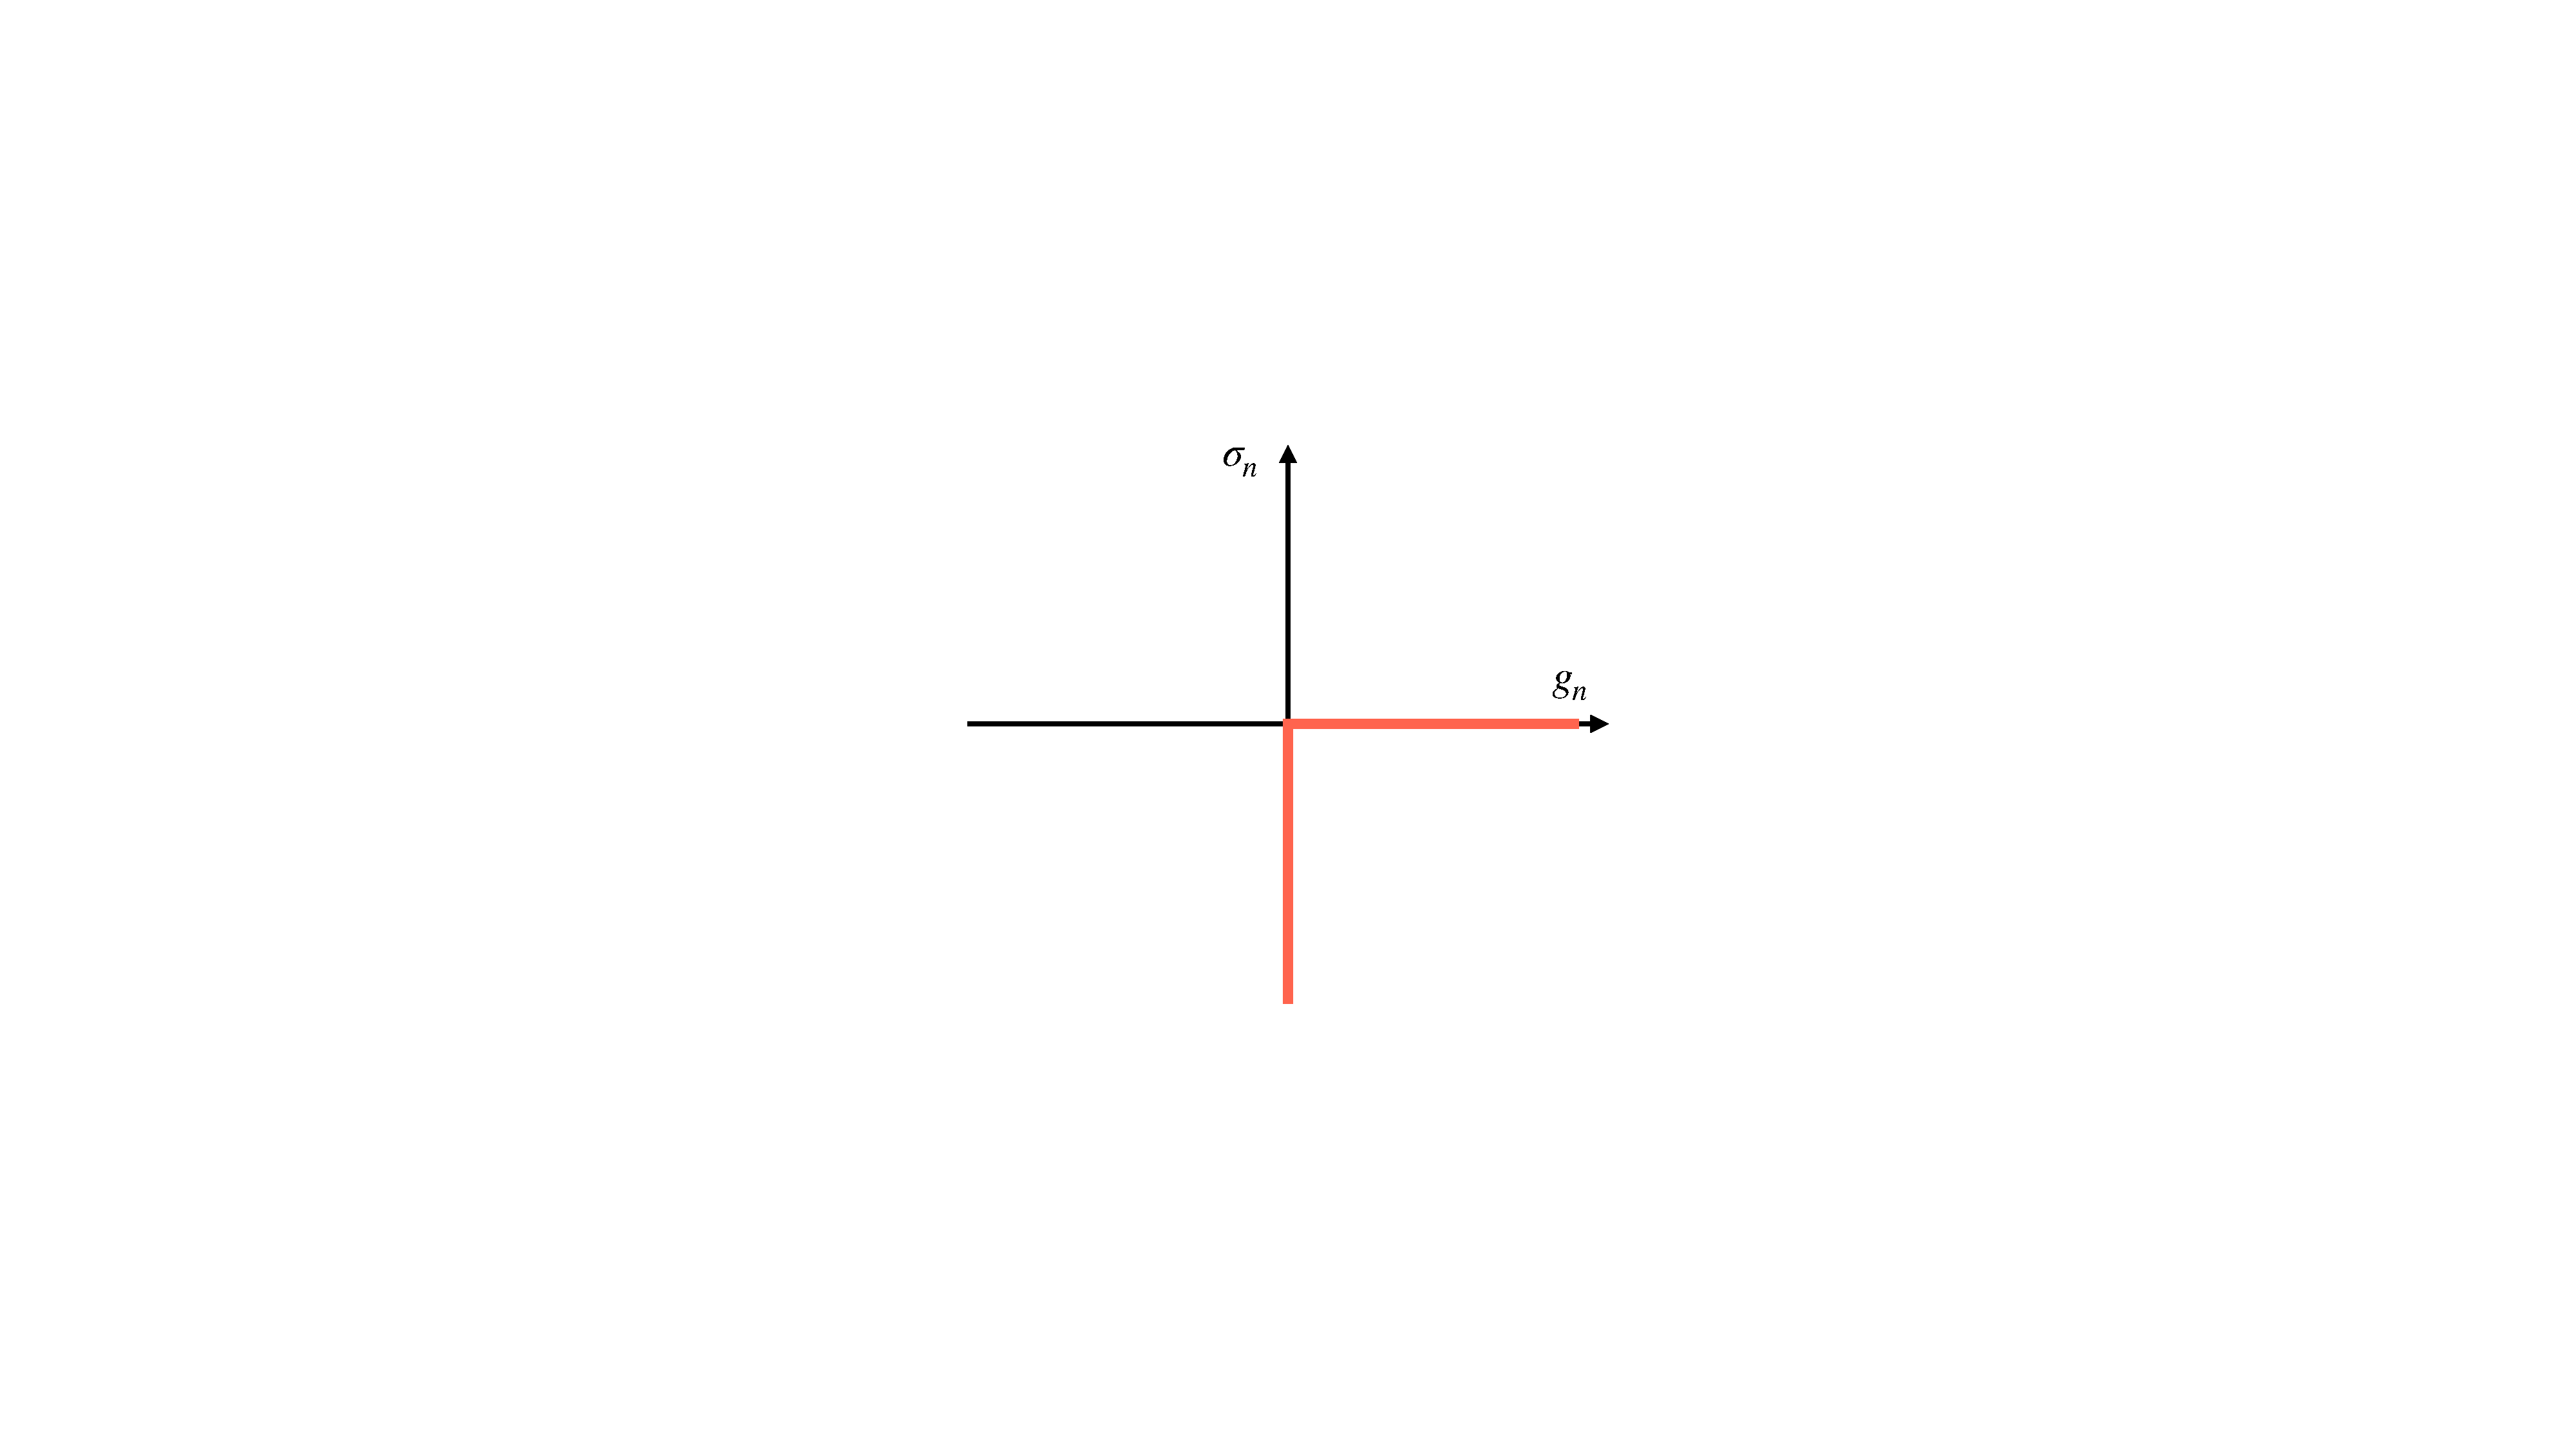
\includegraphics[scale=0.43]{Chapter1/Pictures/signorini.pdf}
    \caption{Illustration of Signorini conditions}
    \label{fig:signori}
\end{figure}

For small deformation problems, the gap function \eqref{gap_fun} can be linearised as follows

\begin{equation}\label{gap_fun}
\Delta g_n = [\bm{u}^{(1)}-\overleftarrow{\bm{u}}^{(2)}].\bm{\hat{\mathrm v}}_{n}+g_0 = u_n+g_0
\end{equation}

where $g_0$ represents the gap function in the reference configuration. Hence, for any incremental time, the linearized expression of the gap function will be used for the following definitions where the condition \eqref{no_penet} can be expressed as  

\begin{equation}
u_n+g_0 \geq 0 \quad \mathrm{or} \quad u_n-g_0 \leq 0
 \end{equation}
 
 We use the later convention  $u_n-g_0 \leq 0$ for the following definitions.


\subsection{Friction formulation}

Friction is defined through Coulomb-Amonton's law where it is based on threshold conditions to define stick and slip characteristics where no motion is allowed until $||\bm\sigma_{t}||$ satisfies the threshold $\mu ||\bm\sigma_{n}||$, defined as follows

\begin{subequations}\label{fric_bc}
\begin{equation}
|\bm{\dot{u}}_t| \geq 0
\end{equation} 

\begin{equation}
||\bm\sigma_{t}||-\mu|\sigma_{n}| \leq 0
\end{equation}

\begin{equation}
 (||\bm\sigma_{t}||-\mu|\sigma_{n}|)|\bm{\dot{u}}_t| = 0
\end{equation}

\end{subequations}

where $\mu$ is the classical coefficient of friction. The above conditions can be interpreted as follows, for the stick condition $|\bm{\dot{u}}_t|=0$,  $||\bm\sigma_{t}||\leq\mu|\sigma_{n}| $ where $||\bm\sigma_{t}||$  is inside Coulomb's cone in the space of traction stresses and similarly for the slip condition $|\bm{\dot{u}}_t|>0$,  $||\bm\sigma_{t}||=\mu|\sigma_{n}| $ where $||\bm\sigma_{t}||$ is on the Coulomb's cone. The conditions are graphically shown in Fig, \ref{fig:Coul_Amon}, similar to Signorini conditions for contact, the conditions define multi-valued mapping. \\

\begin{figure}
    \centering
    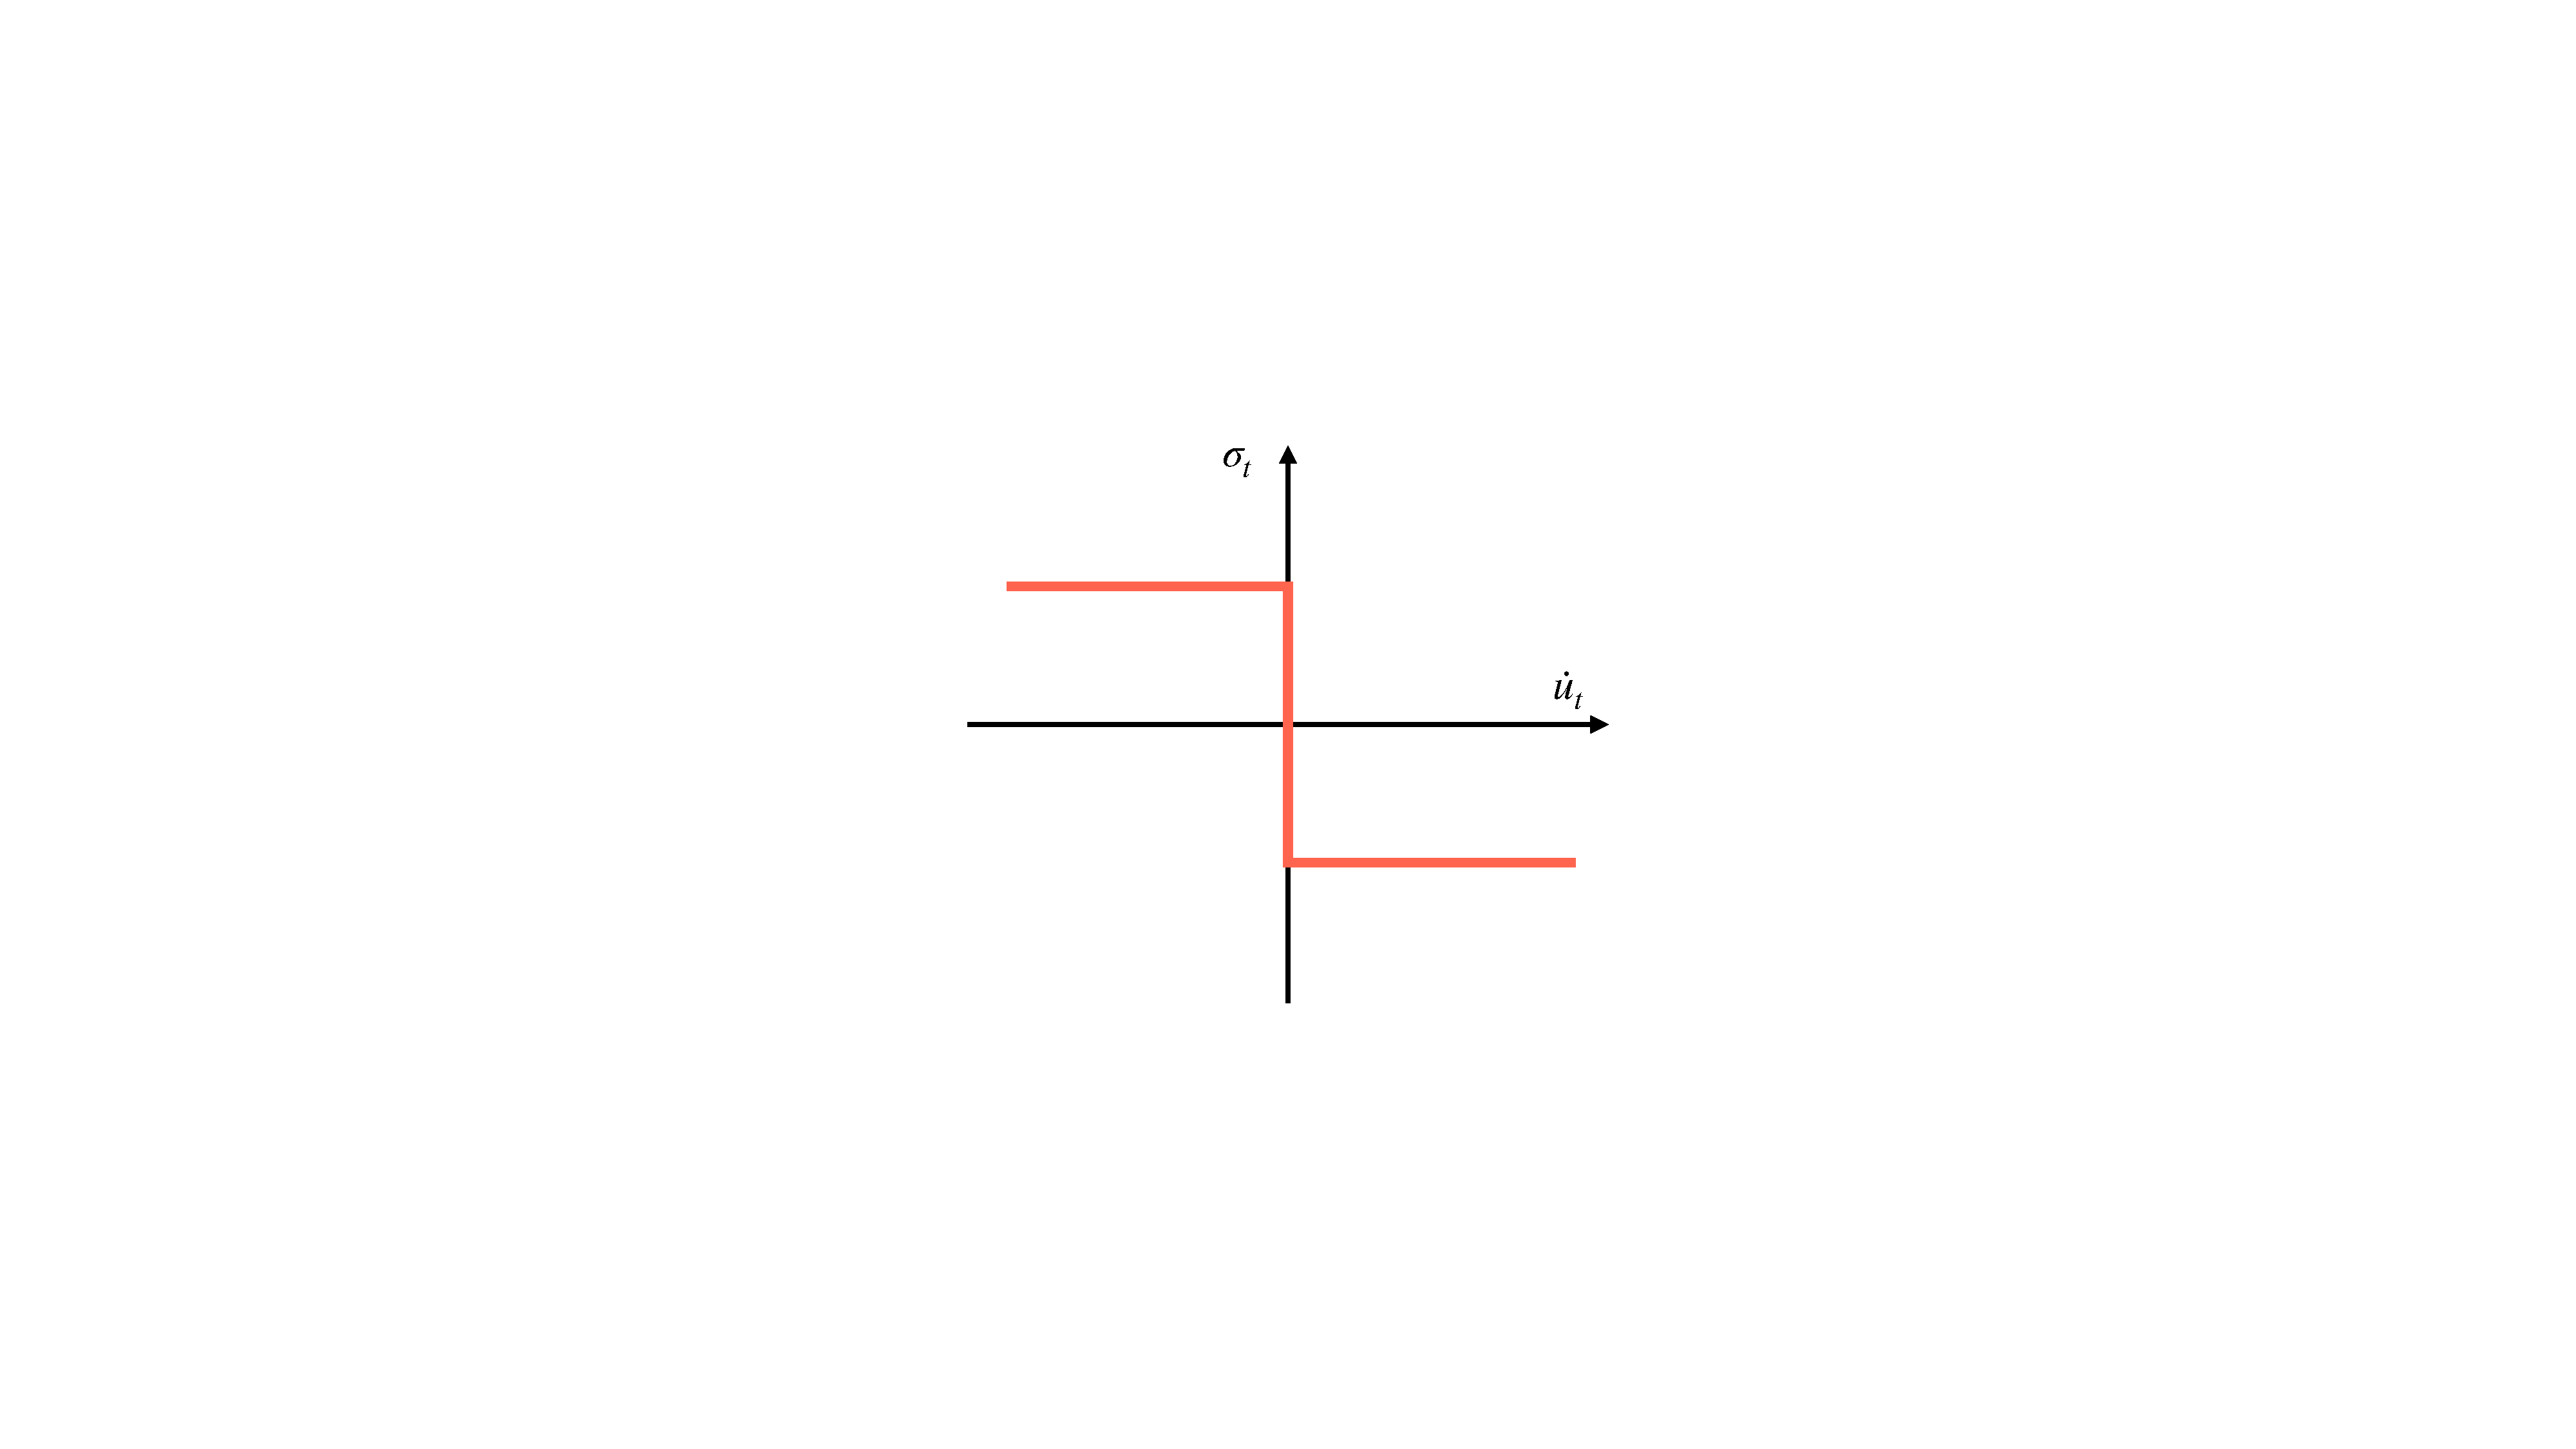
\includegraphics[scale=0.43]{Chapter1/Pictures/Coul_Amon.pdf}
    \caption{Illustration of Coulomb-Amonton's law for friction}
    \label{fig:Coul_Amon}
\end{figure}


The initial boundary value problem Eq.\eqref{cont_eq1} with unilateral conditions for contact and friction can be given as follows

\begin{equation}\label{cont_eq2}
\begin{split}
\rho\bm{\ddot{u}}+\nabla.\bm{\sigma}(\bm{u}) = \bm{f}\quad \mathrm{in} \quad \Omega\\ 
\bm{u} = \bm{u}_D\quad \mathrm{on}\quad \Gamma_D\\
\bm{\sigma}(\bm{u}).\bm{\hat{\mathrm v}}_n=\bm{t}_N\quad\mathrm{on}\quad\Gamma_N\\
%\bm{\sigma}_\mathrm{k}(u_\mathrm{k}).\hat{\mathrm v}_t=F_{f_\mathrm{k}}\quad\mathrm{on}\quad\Gamma_{c,\mathrm{k}}\\\
\\
g_n \geq 0,\quad {\sigma}_n \leq 0,\quad g_n {\sigma}_{n} = 0\quad \\
|\bm{\dot{u}}_t| = 0 \implies ||\bm\sigma_{t}||-\mu|\sigma_{n}| \leq 0\\
|\bm{\dot{u}}_t| \neq 0 \implies ||\bm\sigma_{t}||-\mu|\sigma_{n}|\frac{\bm{\dot{u}}_t}{|\bm{\dot{u}}_t|} = 0\\
\mathrm{on} \quad \Gamma_C\\
\end{split}
\end{equation}


Unlike the classical weak form \eqref{weak_f} which can be obtained through the optimisation of minimising the energy functional, the presence of inequalities from contact and friction expresses the problem in the context of convex optimisation of functional.  Hence, the weak form of the problem has the form of variational inequality where the admissible solution $\bm{\dot{u}}$ is defined over a convex set, given as follows



\begin{multline}\label{fric_con_raw}
\int_{\Omega}\rho\bm{\ddot{u}}.(\delta \bm{u}-\bm{\dot{u}}) \,\ d\Omega +\int_{\Omega}  \bm{\sigma}(\bm{u}):(\nabla \delta \bm{u}-\nabla \bm{\dot{u}}) \,\,d\Omega\\
 - \int_{\Gamma_C} \sigma_n(\delta{u}_n-{\dot{u}}_n) \,\, d\Gamma_C - \int_{\Gamma_C} \sigma_t(|\delta{\bm{u}}_t|-|{\dot{\bm{u}}}_t|) \,\, d\Gamma_C\\
  -  \int_{\Gamma_N} \bm{t}_N.(\delta \bm{u}-\bm{\dot{u}}) \,\, d\Gamma_N- \int_{\Omega} \bm{f}.(\delta \bm{u}-\bm{\dot{u}}) \,\, d\Omega \geq 0
\end{multline}


where the weak form contains the simultaneous presence of two inequalities for contact and friction. To make it complete as an initial boundary value problem, the initial conditions can be defined as $\bm{u}_0$ and $\bm{\dot{u}}_0$ which satisfies the above equation at the initial time. \\
% the function space 

The solution to the above dynamical problem is often discussed in the context of non-smooth mechanics which we do not focus here. 
%Discuss existence of sol
%The above problem characterizes rigid body motion where the solution may not be ensured. 
%The problem is often given as a quasi-static variation, where 
The existence and uniqueness of solution to the above problem  is conferred under certain conditions through regularisation of the multi-valued mapping from the Signorini conditions \eqref{cont_bc} and the Coulomb-Amonton's law \eqref{fric_bc} . Such multi-valued mapping are also seen as fundamental in defining some of the friction-induced dynamic instabilities such as stick-slip. Hence, the model for regularization and the parameters in modelling the regularization are important depending on the hypotheses that model the nature of a given instability.\\ 

We focus on modelling flutter-type dynamic instability through classical theories of linear analysis, where the effect of perturbation around a fixed point is analysed. Hence, the stability of the dynamical system with frictional contact \eqref{fric_con_raw} can be characterized by determining the fixed point which is typically quasi-static or steady-sliding equilibrium depending on the characteristics of the external forces, and defining the dynamics for the perturbation around the fixed point.
For non-linear systems such as the system with frictional contact, the stability can be defined through linearizing the perturbation around a fixed point, which brings the question of modelling the multi-valued mapping to be linear. 
This is possible through regularization of the multi-valued mapping with functions through normal-compliance approach which will be discussed in detail with the case of steady-sliding equilibrium.   
As an intermediate step in realizing the stability analysis for the steady-sliding equilibrium, we discuss the quasi-static insight for the above dynamical system \eqref{fric_con_raw}.\\


The dynamical problem can be expressed as quasi-static problem when the inertial effects can be ignored, given as 

\begin{multline}\label{fric_con_quasi}
\int_{\Omega}  \bm{\sigma}(\bm{u}):(\nabla \delta \bm{u}-\nabla \bm{\dot{u}}) \,\,d\Omega\\
 - \int_{\Gamma_C} \sigma_n(\delta{u}_n-{\dot{u}}_n) \,\, d\Gamma_C - \int_{\Gamma_C} \sigma_t(|\delta{\bm{u}}_t|-|{\dot{\bm{u}}}_t|) \,\, d\Gamma_C\\
  -  \int_{\Gamma_N} \bm{t}_N.(\delta \bm{u}-\bm{\dot{u}}) \,\, d\Gamma_N- \int_{\Omega} \bm{f}.(\delta \bm{u}-\bm{\dot{u}}) \,\, d\Omega \geq 0
\end{multline}
 
The quasi-static frictional problem characterizes the time-dependent variation of $\bm{u}_t$ with Coulomb's conditions, which implies the presence of time-dependent external forces $\bm{t}_N$ and $\bm{f}$. Hence, the system can be considered as series of quasi-static equilibrium, where the stability of the dynamical system can be characterized around such equilibrium states. 
This means that the stability could be defined taking in to account of the time-dependent external forces, or also velocity-dependent friction coefficient, where the history of loading is important for such applications. The solution to the quasi-static problem, either with uniqueness or non-uniqueness is proved to exist under strict conditions.\\

The quasi-static equilibrium can be expressed as a steady-sliding equilibrium between at least two half-spaces when no net acceleration is present. Similar to quasi-static equilibrium, this can be seen as a series of equilibrium states with respect to time where the equilibrium characteristics remain the same, except for the change in the contact domain. Since the equilibrium characteristics remain the same for all the time, the equilibrium state could be expressed with no time dependent forces but purely by static forces. This also means that the knowledge of $\bm{\hat{\mathrm v}}_t$ for ${\sigma}_t\bm{\hat{\mathrm v}}_t$ at $\Gamma_C$ is known a priori, where the general notion of  $\bm{\hat{\mathrm v}}_t$ could be given as  $\bm{\hat{\mathrm v}}_k$ for the known sliding direction. Hence, the time-independent definition of Coulomb's law could be expressed for the so-called static state as follows

\begin{subequations}
\begin{equation}
|\bm{{u}}_t| \geq 0
\end{equation} 

\begin{equation}
||\bm\sigma_{t}||-\mu|\bm\sigma_{n}| \leq 0
\end{equation}

\begin{equation}
 (||\bm\sigma_{t}||-\mu|\bm\sigma_{n}|)|\bm{{u}}_t| = 0
\end{equation}

\end{subequations}
   

The steady-sliding equilibrium explicitly defines the slip condition where the sliding velocity is constant and hence at the equilibrium, $\sigma_t = \mu\sigma_n $ at $\Gamma_C$. 
For simplicity, we consider only one half-space of the sliding contact where the half-space is considered to be fixed relative to the other half-space, while the other half-space moves parallel to $\bm{\hat{\mathrm v}}_t$ creating a sliding contact.
Hence, at any time, the equilibrium state could be expressed as follows

\begin{multline}
\int_{\Omega}  \bm{\sigma}(\bm{u}):(\nabla \delta \bm{u}-\nabla \bm{{u}}) \,\,d\Omega - \int_{\Gamma_C} \mu\sigma_n(|\delta{\bm{u}}_t|-|{{\bm{u}}}_t|) \,\, d\Gamma_C\\
  -  \int_{\Gamma_N} \bm{t}_N.(\delta \bm{u}-\bm{{u}}) \,\, d\Gamma_N- \int_{\Omega} \bm{f}.(\delta \bm{u}-\bm{{u}}) \,\, d\Omega \geq 0
\end{multline}

Since the knowledge of $\bm{\hat{\mathrm v}}_t$ for ${u}_t\bm{\hat{\mathrm v}}_t$ at $\Gamma_C$ is known a priori as $\bm{\hat{\mathrm v}}_k$ and with the slip condition for friction, the above formulation can be defined as follows

\begin{multline}\label{pre_normcomp}
\int_{\Omega}  \bm{\sigma}(\bm{u}):(\nabla \delta \bm{u}-\nabla \bm{{u}}) \,\,d\Omega - \int_{\Gamma_C} \mu\sigma_n(\delta \bm{u}-\bm{{u}}).\bm{\hat{\mathrm v}}_k \,\, d\Gamma_C\\
  -  \int_{\Gamma_N} \bm{t}_N.(\delta \bm{u}-\bm{{u}}) \,\, d\Gamma_N- \int_{\Omega} \bm{f}.(\delta \bm{u}-\bm{{u}}) \,\, d\Omega \geq 0
\end{multline}

where the multi-valued mapping of friction is replaced by a smooth definition. We now introduce the function space for defining $\delta \bm{u}$ and $\bm{{u}}$, where $\delta \bm{u}$ and $\bm{{u}}$ are defined to be from the same space $\bm K\subset \bm V $, with $\bm K$ being the convex subset of $\bm V$, given as\\

\qquad$\bm V:= \{ \delta \bm{u} \in (H^1(\Omega))^3 | \delta \bm{u}=\bm{u}_D\,\, \mathrm{on} \,\, \Gamma_D\}$\\

\qquad $\bm K:=\{\delta \bm{u} \in \bm V | \delta \bm{u}_n \leq g_n\}$\\

\qquad $\bm{f}\in (L^2(\Omega))^3$ and $\bm{t} \in (H^{-1/2}(\partial\Omega))^3$\\

where $(H^1(\Omega))^3$ is the Sobolev space of functions, given with the property\\ 

$(H^1(\Omega))^3 := \{ \delta \bm u \in (L^2(\Omega))^3, \nabla\delta \bm u  \in (L^2(\Omega))^3 \}$\\ 

Hence, the Hilbert space induced by inner product is given through $L^2$ norm:
  
${\|{\delta \bm u}\|_{L^2}= \langle {\delta \bm u},{\delta \bm u} \rangle=\int_{\Omega} {\delta \bm u}^2 d\Omega < \infty }$. A subspace $(H^{1/2}(\partial\Omega))^3$ can be defined as the restriction of $(H^{1}(\Omega))^3$ on $\partial\Omega$, where $(H^{-1/2}(\partial\Omega))^3$ is the dual of the space $(H^{1/2}(\partial\Omega))^3$.

Even though  $\bm{t}$ is typically defined to be in $L^2(\Omega)$, the unknown a priori conditions of $\bm{t}$ for $\sigma_n$ on $\Gamma_C$ results in the space to be $H^{1/2}(\partial\Omega)$.
Unlike the case for the dynamical problem or quasi-static problems which are characterized by the presence of two simultaneous inequalities, the above problem is characterized purely by the inequalities of the Signorini conditions, when friction is defined for the slip condition with equality.\\

The Signorini and Coulomb's conditions \eqref{cont_bc} \eqref{fric_bc} represent the mathematical model for contact and friction in macroscopic view, where such conditions have been found through experiments to be far from the physical reality. This leads to the view of normal compliance approach to define a better approximation of the physical reality, also through which regularization for the muti-valued mappings is achieved, where $\sigma_n$ is related as the function of gap function $g_n$ with a set of parameters determined largely by experiments, given as  

\begin{equation}\label{normal_comp}
-\sigma_n = c_n(u_n-g_n)_+^{m_n}
\end{equation}

where  $(.)_+$ allows only positive value. This can be extended to friction as follows

\begin{subequations}
\begin{equation}
|\bm{\dot{u}}_t| \geq 0
\end{equation} 

\begin{equation}
||\bm\sigma_{t}||-c_t(u_n-g_n)_+^{m_t} \leq 0
\end{equation}

\begin{equation}
 ||\bm\sigma_{t}||-c_t(u_n-g_n)_+^{m_t} |\bm{\dot{u}}_t| = 0
\end{equation}

\end{subequations}

where the parameters $c_n$, $m_n$, $c_t$ and $m_t$ are determined from the experiments. 
The normal compliance can also be applied to the previously defined dynamic and quasi-static cases, where existence and uniqueness of solution were proved through normal compliance under certain assumptions. 
For steady-sliding equilibrium, $|\bm{\dot{u}}_t|$ can be expressed as $|\bm{{u}}_t|$.\\

The Eq. \eqref{pre_normcomp} can hence be defined through normal compliance as follows

\begin{multline}
\int_{\Omega}  \bm{\sigma}(\bm{u}):(\nabla \delta \bm{u}-\nabla \bm{{u}}) \,\,d\Omega - \int_{\Gamma_C} c_t(u_n-g_n)_+^{m_t}(\delta \bm{u}-\bm{{u}}).\bm{\hat{\mathrm v}}_k \,\, d\Gamma_C\\
  -  \int_{\Gamma_N} \bm{t}_N.(\delta \bm{u}-\bm{{u}}) \,\, d\Gamma_N- \int_{\Omega} \bm{f}.(\delta \bm{u}-\bm{{u}}) \,\, d\Omega \geq 0
\end{multline}

The above variational inequality can be expressed as variational equality through active set strategy, where instead of looking for the admissible displacement field that satisfies the condition ${u}_n \leq g_n$ on $\Gamma_C$, as the minimizer of the above functional in the convex set $\bm K$ if there exists a unique solution in the set, the set $\Gamma_C$ is defined a priori, called active set, at least for an incremental time for which ${u}_n  - g_n \rightarrow 0$, provided that ${u}_n \leq g_n$ was satisfied prior to the given time. 
With the knowledge of active set, the displacement field $u_n$ on $\Gamma_C$ could be satisfied by normal compliance given in Eq. \eqref{normal_comp}.
Hence, the above functional with inequality can be expressed through equality as follows

 \begin{multline}\label{SS_pen}
\int_{\Omega}  \bm{\sigma}(\bm{u}):\nabla \delta \bm{u} \,\,d\Omega - 
\underbrace{\int_{\Gamma_C} c_t(u_n-g_n)_+^{m_t}\delta \bm{u}.\bm{\hat{\mathrm v}}_k \,\, d\Gamma_C}_{{\langle \bm{\sigma}_n, \delta \bm u \rangle}} 
+ \underbrace{\int_{\Gamma_C} c_n(u_n-g_n)_+^{m_n}\delta \bm{u}.\bm{\hat{\mathrm v}}_n \,\, d\Gamma_C}_{{\langle \bm{\sigma}_t, \delta \bm u \rangle}}\\
  -  \int_{\Gamma_N} \bm{t}_N.\delta \bm{u} \,\, d\Gamma_N- \int_{\Omega} \bm{f}.\delta \bm{u} \,\, d\Omega = 0
\end{multline}

where the inner products ${\langle \bm{\sigma}_n, \delta \bm u \rangle}$ and ${\langle \bm{\sigma}_t, \delta \bm u \rangle}$ define the  weak form of contact and friction respectively. 
The definition of $\Gamma_C$ through the active set strategy means that $\bm{t}_N \in (L^2(\Omega))^3$. 
 When $m_n \neq 1$ and $m_t \neq 1$, the steady-sliding equilibrium can be solved through non-linear programming like Newton-Rhapson for $\bm{u}_{eq}$.\\ 
 
We do not relate to the experimental determination of the parameters $c_n$, $m_n$, $c_t$ and $m_t$. Hence, $c_n$ is purely given as the penalty parameter $\mathit{p}$ considering numerical stability, which implies that for any $(u_n-g_0) > 0$ defined by $(u_n-g_0)_+$ is penalized by a factor $p$, where the ideal would be $ \mathit{p} \rightarrow \infty$. 
While $c_t$ is given for the ideal slip state of the steady-sliding equilibrium as $c_t=\mu\mathit{p}$. 
The normal compliance approach can be viewed in general as modelling springs with certain stiffness $c_n$ which resist penetration at the contact interface. 
We consider $m_n = m_t = 1$, where the parameters $m_n$ and $m_t$ for any value other than $1$ can be physically interpreted as non-linear springs. 
With the above consideration of the parameters for the normal compliance, the above functional can be expressed as follows

 \begin{multline}\label{SS_pen_1}
\int_{\Omega}  \bm{\sigma}(\bm{u}):\nabla \delta \bm{u} \,\,d\Omega - \int_{\Gamma_C} \mu\mathit{p}(u_n-g_n)_+\delta \bm{u}.\bm{\hat{\mathrm v}}_k \,\, d\Gamma_C + \int_{\Gamma_C} \mathit{p}(u_n-g_n)_+\delta \bm{u}.\bm{\hat{\mathrm v}}_n \,\, d\Gamma_C\\
  -  \int_{\Gamma_N} \bm{t}_N.\delta \bm{u} \,\, d\Gamma_N- \int_{\Omega} \bm{f}.\delta \bm{u} \,\, d\Omega = 0
\end{multline}




where for finite deformation, the problem can be solved for $\bm{u}_{eq}$ with one incremental time step.\\

The perturbed state of the displacement field for any excitation of the steady-sliding equilibrium can be given as 

\begin{equation}\label{pert_wrt_eq}
\bm{u}=\bm{u}_{eq}+\bm{\widetilde{u}}
\end{equation}

 where $\bm{\widetilde{u}}$ corresponds to the perturbed displacement field. The idea is to analyse the dynamics of the perturbation such that the stability of the dynamical system can be determined through the onset evolution of the dynamics for the perturbation, where it is hypothesized that the onset evolution of the dynamics can be expressed linearly. This brings the question of linearization for the non-linear frictional contact problem, even with the sufficient approximation made for Eq. \eqref{SS_pen_1}.\\

 As a detour for generalization, we discuss the linearization of the normal compliance terms. The contact and friction terms in Eq. \eqref{SS_pen} with $c_n=p, c_t=\mu p$, $0< m_n \neq 1$  and $0< m_t \neq 1$ , can be expressed as\\ 
 
 \begin{subequations}\label{genli}
 \begin{equation}
 {\langle \bm{\sigma}_n, \delta \bm u \rangle_{\Gamma_C}}=\int_{\Gamma_C} \mathit{p}(u_n-g_0)^{m_n}_+\delta \bm{u}.\bm{\hat{\mathrm v}}_n \,\, d\Gamma_C
  \end{equation}
  \begin{equation}
  {\langle \bm{\sigma}_t, \delta \bm u \rangle_{\Gamma_C}}= \int_{\Gamma_C} \mu\mathit{p}(u_n-g_0)^{m_t}_+\delta \bm{u}.\bm{\hat{\mathrm v}}_k \,\, d\Gamma_C
  \end{equation}
 \end{subequations}
 
 
% when $m_n \neq 1$ and $m_t \neq 1$, the steady-sliding equilibrium can be solved through non-linear programming like Newton-Rhapson for $\bm{u}_{eq}$.\\ 
 
 The perturbation of the normal compliance can hence be expressed as\\
 
  \begin{subequations}
 \begin{equation}
 \mathit{p}(\widetilde{u}_n+u_n-g_n)^{m_n}_+- \mathit{p}(u_n-g_0)^{m_n}_+\approx \mathit{p}(\widetilde{u}_n)^{m_n}_+
   \end{equation}
    \begin{equation}
 \mu\mathit{p}(\widetilde{u}_n+u_n-g_n)^{m_t}_+- \mu\mathit{p}(u_n-g_0)^{m_t}_+\approx \mu\mathit{p}(\widetilde{u}_n)^{m_t}_+
    \end{equation}
  \end{subequations}
  
 if it can be assumed that the parameters of the normal compliance stay the same for the perturbation $\bm{\widetilde{u}}$ close to the equilibrium $\bm{u}_{eq}$. The linearization for the degree of the polynomial terms at $\bm{u}_{eq}$ can be defined as\\
 
 \begin{subequations}
 \begin{equation}
  \Delta \mathit{p}(\widetilde{u}_n)^{m_n}_+ |_{\bm{u}_{eq}}
 = m_n \mathit{p}(\widetilde{u}_n)^{m_n-1}_+|_{\bm{u}_{eq}}
 \end{equation}
  \begin{equation}
   \Delta \mu\mathit{p}(\widetilde{u}_n)^{m_t}_+ |_{\bm{u}_{eq}}
   = \mu m_t \mathit{p}(\widetilde{u}_n)^{m_t-1}_+|_{\bm{u}_{eq}}
  \end{equation}
 \end{subequations}
 
where the expressions are still non-linear in the presence of $(.)_+$. It should be noted that the perturbation $\widetilde{u}_n$ on $\Gamma_C$ may not result in the same active set as the equilibrium, due to the possible separation at some parts on $\Gamma_C$, which introduces non-linearities defined by $(.)_+$. 
 This is because the separation leads to $u_n-g_0 < 0$ and hence $p(u_n-g_0)_+^{m_n} \rightarrow 0$ which can only be taken in to account nonlinearly. 
 This is linearized with the hypothesis that the onset of instability occurs very close to the equilibrium $\bm{u}_{eq}$ such that $\Gamma_C$ remains the same for the perturbation $\bm{\widetilde{u}}$. This means that if $\Gamma_C$ must be constant for $\widetilde{\bm{u}}$, the separation $u_n-g_0 < 0$ must also be penalized which can simply be achieved by evading the operator $(.)_+$ .  
The above hypothesis for the perturbation of $\widetilde{u}_n$ on $\Gamma_C$ would have been impossible to define with Signorini conditions where $\widetilde{u}_n$ may lead to strict contact separation on $\Gamma_C$, while in the view of normal compliance, the perturbation $\widetilde{u}_n$ for no variation of $\Gamma_C$ can be considered to  define the variation of $\sigma_n$ and hence also its subsequent effect on $\sigma_t$ for friction.\\
  
With the above hypothesis, the linearized weak form of contact and friction for the dynamics of the perturbation $\bm{\widetilde{u}}$ close to $\bm{u}_{eq}$ can be defined as\\
 
 \begin{subequations}
 \begin{equation}
 {\langle \bm{\sigma}_n, \delta \bm u \rangle_{\Gamma_C}}= \int_{\Gamma_C} m_n\mathit{p}{\widetilde{u}_n}^{\,m_n-1}|_{\bm{u}_{eq}}\delta \bm{u}.\bm{\hat{\mathrm v}}_n \,\, 
 d\Gamma_C
 \end{equation}
 \begin{equation}
  {\langle \bm{\sigma}_t, \delta \bm u \rangle_{\Gamma_C}}=\int_{\Gamma_C} \mu m_n\mathit{p}{\widetilde{u}_n}^{\,m_n-1}|_{\bm{u}_{eq}}\delta \bm{u}.\bm{\hat{\mathrm v}}_k \,\, d\Gamma_C\\
 \end{equation}
 \end{subequations}
 %This can be assumed that the $c_n = p$ and $c_n = p$ is purely determined 
It should be noted that the above weak form is different from the classical weak form of contact and friction defined by normal compliance in Eq. \eqref{SS_pen}. The above weak form essentially characterises force which is purely displacement-dependent, also known as follower force. The definition of follower force can be largely said as implicit for modelling flutter-type dynamic instability. 
In the case of flutter-type instability arising from friction between solids, the main hypothesis is that the onset of instability occurs at perturbations very close to $\bm u_{eq}$ such that the non-linearities of the classical contact and friction \eqref{SS_pen} can be effectively ignored and hence, friction phenomenon for a perturbed state $\widetilde{\bm u}$ can be modelled linearly with the contact state of $\bm u_{eq}$ purely by displacement-dependent forces.
Hence, the hypothesis only characterises $\widetilde{\bm u}$ with the linearization of non-linearities very close to $\bm u_{eq}$, while the characteristics of non-linearities away from $\bm u_{eq}$ cannot be forseen.
This essentially reflects on the possibility of utilising linear analysis such as CEA \ref{Phy_CEA}, where CEA can characterise instability of a system through eigenmodes in one computation, which would otherwise require expensive transient analysis to find a limit cycle.
This defines the system to be holonomic and autonomous since the nature of follower force depends only on generalized coordinates without explicit time dependence. 
%It should be noted that linearization effectively models instabilities very close to the equilibrium, while the effect of non-linearities away from $\bm u_{eq}$ is not present. \\

We consider the case of $m_n = 1$ and $m_t = 1$ for the following discussions, where the linearization of Eqs. \eqref{genli} can simply be expressed as\\ 
 
 \begin{subequations}
 \begin{equation}
 {\langle \bm{\sigma}_n, \delta \bm u \rangle_{\Gamma_C}}= \int_{\Gamma_C} \mathit{p}{\widetilde{u}_n}\delta \bm{u}.\bm{\hat{\mathrm v}}_n \,\, d\Gamma_C
   \end{equation}
   \begin{equation}
  {\langle \bm{\sigma}_t, \delta \bm u \rangle_{\Gamma_C}}= \int_{\Gamma_C} \mu \mathit{p}{\widetilde{u}_n}\delta \bm{u}.\bm{\hat{\mathrm v}}_k \,\, d\Gamma_C
     \end{equation}
   \end{subequations}
   
 The initial-boundary value problem for the dynamics of the perturbation can be given as
 
\begin{equation}\label{pert_dyn}
\begin{split}
\rho^\mathrm{(k)}\bm{\ddot{\widetilde{u}}}^\mathrm{(k)} +\nabla\bm{.}\bm{\sigma}^\mathrm{(k)}(\bm{\widetilde u}^\mathrm{(k)}) = 0 \quad \mathrm{in} \quad \Omega^\mathrm{(k)}\\ 
\bm{\widetilde u}^\mathrm{(k)} = \bm{\widetilde u}^\mathrm{(k)}_{D} \quad \mathrm{on}\quad\Gamma^{\mathrm{(k)}}_D\\
\sigma^{(\mathrm k)}_n(\bm{\widetilde u}^\mathrm{(k)}) \bm{\hat{\mathrm v}}_n = - \mathit{p}{\widetilde{u}_n}^{(\mathrm k)} \bm{\hat{\mathrm v}}_n,\quad \sigma^{(\mathrm k)}_t(\bm{\widetilde u}^\mathrm{(k)})  \bm{\hat{\mathrm v}}_k = \mu \mathit{p}{\widetilde{u}_n}^{(\mathrm k)} \bm{\hat{\mathrm v}}_k \quad \mathrm{on}\quad\Gamma^{\mathrm{(k)}}_C\\
%\bm{\sigma}_\mathrm{k}(u_\mathrm{k}).\hat{\mathrm v}_t=F_{f_\mathrm{k}}\quad\mathrm{on}\quad\Gamma_{c,\mathrm{k}}\\
\end{split}
\end{equation}

It should be noted that for linear case, the problem can be explicitly defined without the fore knowledge of $\bm u_{eq}$, by defining $\Gamma_C$ explicitly. For simplicity, we consider the parameters $p$ and $\mu$ to be constant between the contact interface of all the domains in contact. The subscript $\mathrm{k}$ distinguishes the domains in contact.  Similar to Eq. \eqref{weak_f}, the weak form of the differential formulation can be expressed as

\begin{equation} \label{weak_pert}
\int_{\Omega^{(k)}}\rho^\mathrm{(k)}\bm{\ddot{\widetilde{u}}}^\mathrm{(k)}. \delta\bm u^\mathrm{(k)} \,\,d\Omega^\mathrm{(k)} +\int_{\Omega^{(k)}} \bm{\sigma}^\mathrm{(k)}(\bm{\widetilde u}^\mathrm{(k)}) : \nabla\delta\bm u^\mathrm{(k)} \,\,d\Omega^\mathrm{(k)} - \int_{\Gamma^{(k)}_C} \bm t_C^\mathrm{(k)}  .  \delta\bm u^\mathrm{(k)} \,\,d\Gamma_{C}^\mathrm{(k)} = 0 
\end{equation}
 
The traction force $\bm t_C \in H^{-{1}/{2}}(\Gamma_C)$ can be decomposed as follows

\begin{equation}
\begin{split}
 \int_{\Gamma^{(\mathrm k)}_C}  \bm t_C^\mathrm{(k)}  .  \delta\bm u^\mathrm{(\mathrm k)}  \,\,d\Gamma_{C}^\mathrm{(k)} = \int_{\Gamma^{(k)}_C} ( \sigma_n^{(\mathrm k)} \bm{\hat{\mathrm v}}_n+  \sigma_t^{(\mathrm k)}\bm{\hat{\mathrm v}}_k) .
 \delta\bm u^\mathrm{(k)} \,\,d\Gamma_{C}^\mathrm{(k)}\\ 
 =  {\int_{\Gamma^{(k)}_C}  \sigma_n^{(\mathrm k)} \bm{\hat{\mathrm v}}_n. \delta\bm u^\mathrm{(k)}} \,\,d\Gamma_{C}^\mathrm{(k)}+ {\int_{\Gamma^{(k)}_C}  \sigma_t^{(\mathrm k)} \bm{\hat{\mathrm v}}_k. \delta\bm u^\mathrm{(k)}} \,\,d\Gamma_{C}^\mathrm{(k)}
 \end{split}
\end{equation}

Hence, the Eq. \eqref{weak_pert} for the $\mathrm n_{\mathrm k}$ domains in contact can be defined as 

\begin{multline} 
\sum_{\mathrm{k}=1}^{\mathrm{n}_{\mathrm{\mathrm{k}}}}   \bigg\{  \int_{\Omega^{(k)}}\rho^\mathrm{(k)}\bm{\ddot{\widetilde{u}}}^\mathrm{(k)}. \delta\bm u^\mathrm{(k)} \,\,d\Omega^\mathrm{(k)}+\int_{\Omega^{(k)}} \bm{\sigma}^\mathrm{(k)}(\bm{\widetilde u}^\mathrm{(k)}) : \nabla \delta\bm u^\mathrm{(k)} \,\,d\Omega^\mathrm{(k)}\\  -    \underbrace{\int_{\Gamma^{(k)}_C}  \sigma_n^{(\mathrm k)} \bm{\hat{\mathrm v}}_n. \delta\bm u^\mathrm{(k)}  \,\,d\Gamma_{C}^\mathrm{(k)}}_{\langle \bm{\sigma}^{\mathrm{(k)}}_n, \delta \bm u^{\mathrm{(k)}} \rangle_{\Gamma_C^{\mathrm{(k)}}}} - \underbrace{\int_{\Gamma^{(k)}_C}  \sigma_t^{(\mathrm k)} \bm{\hat{\mathrm v}}_k. \delta\bm u^\mathrm{(k)}  \,\,d\Gamma_{C}^\mathrm{(k)}}_{\langle \bm{\sigma}^{\mathrm{(k)}}_t, \delta \bm u^{\mathrm{(k)}} \rangle_{\Gamma_C^{\mathrm{(k)}}}} \bigg\} = 0 
\end{multline}\label{weak_pert_1}

where $\bm \sigma_n, \bm \sigma_t \in (H^{-1/2}(\Gamma_C))^3$.  The inner products can be expressed in $(H^{1/2}(\Gamma_C))^{3}$ space which is the restriction of $\bm u \in H^{1}(\Omega) \rightarrow H^{1/2} (\Gamma_C)$  through the normal compliance approach, where the above equation can be defined as  

\begin{multline}  
\sum_{\mathrm{k}=1}^{\mathrm{n}_{\mathrm{\mathrm{k}}}}   \bigg\{  \int_{\Omega^{(k)}}\rho^\mathrm{(k)}\bm{\ddot{\widetilde{u}}}^\mathrm{(k)}. \delta\bm u^\mathrm{(k)} \,\,d\Omega^\mathrm{(k)}+\int_{\Omega^{(k)}} \bm{\sigma}^\mathrm{(k)}(\bm{\widetilde u}^\mathrm{(k)}) : \nabla \delta\bm u^\mathrm{(k)} \,\,d\Omega^\mathrm{(k)}\\  
+ \underbrace{\int_{\Gamma^{(k)}_C}  \mathit{p}{\widetilde{u}_n}^{(\mathrm k)} \bm{\hat{\mathrm v}}_n. \delta\bm u^\mathrm{(k)}  \,\,d\Gamma_{C}^\mathrm{(k)}}_{\langle \bm{\sigma}^{\mathrm{(k)}}_n, \delta \bm u^{\mathrm{(k)}} \rangle_{\Gamma_C^{\mathrm{(k)}}}} 
- \underbrace{\int_{\Gamma^{(k)}_C} \mu \mathit{p}{\widetilde{u}_n}^{(\mathrm k)} \bm{\hat{\mathrm v}}_k. \delta\bm u^\mathrm{(k)}  \,\,d\Gamma_{C}^\mathrm{(k)}}_{\langle \bm{\sigma}^{\mathrm{(k)}}_t, \delta \bm u^{\mathrm{(k)}} \rangle_{\Gamma_C^{\mathrm{(k)}}}} \bigg\} = 0 
\end{multline}

For simplicity in expansion of the contact and friction compliance terms, we consider contact between two domains $\Omega^{(a)}$ and $\Omega^{(b)}$, with the derivation of traction forces on $\Omega^{(a)}$. Hence, the inner products ${\langle \bm{\sigma}^{\mathrm{(a)}}_n, \delta \bm u^{\mathrm{(a)}} \rangle_{\Gamma_C^{\mathrm{(a)}}}}$ and ${\langle \bm{\sigma}^{\mathrm{(a)}}_t, \delta \bm u^{\mathrm{(a)}} \rangle_{\Gamma_C^{\mathrm{(a)}}}}$ can be expressed as
 
\begin{equation}\label{pert_cont}
{\langle \bm{\sigma}^{\mathrm{(a)}}_n, \delta \bm u^{\mathrm{(a)}} \rangle_{\Gamma_C^{\mathrm{(a)}}}} = 
\int_{\Gamma^{(\mathrm a)}_C}  \mathit{p}{\widetilde{u}_n}^{(\mathrm a)} \bm{\hat{\mathrm v}}_n. \delta\bm u^\mathrm{(a)} \,\,d\Gamma_{C}^\mathrm{(a)}=
\int_{\Gamma^{(\mathrm a)}_C}  \mathit{p}[({\widetilde{\bm u}}^{(\mathrm a)} - {\widetilde{\bm u}}^{(\mathrm b)}). \bm{\hat{\mathrm v}}_n]  \delta\bm u^\mathrm{(a)}. \bm{\hat{\mathrm v}}_n \,\,d\Gamma_{C}^\mathrm{(a)}
\end{equation}

\begin{equation}\label{pert_fric}
{\langle \bm{\sigma}^{\mathrm{(a)}}_t, \delta \bm u^{\mathrm{(a)}} \rangle_{\Gamma_C^{\mathrm{(a)}}}} = 
\int_{\Gamma^{(\mathrm a)}_C}  \mu \mathit{p}{\widetilde{u}_n}^{(\mathrm a)} \bm{\hat{\mathrm v}}_n. \delta\bm u^\mathrm{(a)} \,\,d\Gamma_{C}^\mathrm{(a)}=
\int_{\Gamma^{(\mathrm a)}_C}  \mu \mathit{p}[({\widetilde{\bm u}}^{(\mathrm a)} - {\widetilde{\bm u}}^{(\mathrm b)}). \bm{\hat{\mathrm v}}_n] \delta\bm u^\mathrm{(a)}. \bm{\hat{\mathrm v}}_k \,\,d\Gamma_{C}^\mathrm{(a)}
\end{equation}

The traction forces on $\Omega^{(b)}$ can similarly be defined from the conservation of momentum as $\bm{\sigma}^{\mathrm{(a)}}_n = - \bm{\sigma}^{\mathrm{(b)}}_n$ and $\bm{\sigma}^{\mathrm{(a)}}_t = - \bm{\sigma}^{\mathrm{(b)}}_t$. 
We defined a suitable function space $\bm V \subset (H^1(\Omega))^3$ on which the solution $\bm u$ of the functional in modelling the continuum is presumed to exist.The arbitrary variation $\delta \bm u$ in an infinite-dimensional function space $\bm V$ can be expressed as

\begin{equation}
\delta \bm u = \sum^{\infty}_\mathrm{i}  \delta \bm \vartheta_\mathrm{i} \bm v_i \qquad \forall  \bm v_i \in \bm V
\end{equation}

Hence, the Eq. \eqref{weak_pert_1} can be defined for a system of two domains $\Omega^{(a)}$ and $\Omega^{(b)}$as 


\begin{multline} \label{weak_pert_2}
\sum^{\mathrm{a,b}}_{\mathrm{k}}    \bigg\{   \bigg( \int_{\Omega^{(k)}}\rho^\mathrm{(k)}\bm{\ddot{\widetilde{u}}}^\mathrm{(k)}.  \bm v_i^\mathrm{(k)} \,\,d \Omega^{(k)}+\int_{\Omega^{(k)}} \bm{\sigma}^\mathrm{(k)}(\bm{\widetilde u}^\mathrm{(k)}) : \nabla \bm v_i^\mathrm{(k)}\,\,d \Omega^{(\mathrm k)}\\  
+\int_{\Gamma^{(k)}_C}  \mathit{p}[({\widetilde{\bm u}}^{(\mathrm k)} - {\widetilde{\bm u}}^{( \sim \mathrm k)}). \bm{\hat{\mathrm v}}_n]  \bm v_i^\mathrm{(k)}. \bm{\hat{\mathrm v}}_n \,\,d{\Gamma^{(k)}_C} 
-\int_{\Gamma^{(k)}_C}  \mu \mathit{p}[({\widetilde{\bm u}}^{(\mathrm k)} - {\widetilde{\bm u}}^{(\sim \mathrm k)}). \bm{\hat{\mathrm v}}_n]  \bm v_i^\mathrm{(k)}. \bm{\hat{\mathrm v}}_k \,\,d{\Gamma^{(\mathrm k)}_C} \bigg) \delta \bm \vartheta  \bigg\} = 0 
\end{multline} 

where the equation must be satisfied for any arbitrary variation of $\delta \bm \vartheta$. $\sim \mathrm k$ defines the domain which is not $\mathrm k$, i.e., $\mathrm{k=a}$ implies $\sim\mathrm{k=b}$ and vice-versa.\\

With the finite element approach, we define a finite-dimensional function space ${}_h \bm {V} \subset \bm V$ and hence, there is some bound for ${}_h \bm v_\mathrm{i} \in {}_h \bm V$. We define the approximation of $\bm u$ in the same space ${}_h \bm V$ as $\bm u \approx {}_h \bm u \in {}_h \bm V$, where the above equation can be defined as

\begin{multline} \label{weak_pert_2}
\sum^{\mathrm{a,b}}_{\mathrm{k}}   \bigg\{ \int_{\Omega^{(k)}}\rho^\mathrm{(k)} {}_h\bm{\ddot{\widetilde{u}}}^\mathrm{(k)}. {}_h \bm v_i^\mathrm{(k)}  \,\,d \Omega^{(\mathrm k)} +\int_{\Omega^{(k)}} \bm{\sigma}^\mathrm{(k)}({}_h \bm{\widetilde u}^\mathrm{(k)}) : \nabla {}_h \bm v_i^\mathrm{(k)} \,\,d \Omega^{(\mathrm k)}\\  
+\int_{\Gamma^{(k)}_C}  \mathit{p}[({{}_h\widetilde{\bm u}}^{(\mathrm k)} - {{}_h \widetilde{\bm u}}^{ (\sim \mathrm k)}). \bm{\hat{\mathrm v}}_n]  {}_h \bm v_i^\mathrm{(k)}. \bm{\hat{\mathrm v}}_n \,\,d{\Gamma^{(\mathrm k)}_C}
-\int_{\Gamma^{(k)}_C}  \mu \mathit{p}[({{}_h\widetilde{\bm u}}^{(\mathrm k)} - {{}_h\widetilde{\bm u}}^{(\sim \mathrm k)}). \bm{\hat{\mathrm v}}_n]  {}_h \bm v_i^\mathrm{(k)}. \bm{\hat{\mathrm v}}_k \,\,d{\Gamma^{(\mathrm k)}_C} \bigg\} = 0 \\
\qquad \forall {}_h \bm v_i^{(\mathrm k)} \in {}_h \bm V^{(\mathrm k)}
\end{multline} 

We explain the definition of space ${}_h \bm V$ for classical finite elements in ~, but we mainly explain in detail for Isogeometric methods with focus on contact in ~, where the Isogeometric approach is new for the given application. 
But given a suitable choice of finite-dimensional space ${}_h \bm V$, the above equation can be defined in matrix form as  

\begin{equation}\label{mat_dyn_fric}
\mathbf M^{(a-b)} \ddot{\bm{\widetilde U}}^{(a-b)} +(\mathbf K^{(a-b)} +\mathbf K_C^{(a-b)}+\mathbf K_F^{(a-b)}) \bm{\widetilde{U}}^{(a-b)} =0
\end{equation}

The properties of the matrices can be given as follows, where $\mathbf M$ and $\mathbf K$ are symmetric and positive definite. $\mathbf K_C$ is also symmetric which essentially defines the conservation of momentum at the interface, while $\mathbf K_F$ is non-symmetric with the non-conservative nature of friction at slip state. 
Often damping matrix $\mathbf C$ is also added purely in numerical context, typically through modal or Rayleigh damping. In the scope of modelling rotational inertia effects, gyroscopic matrix $\mathbf G$ can also be defined, where $\mathbf {C}$ and  $\mathbf {G}$ are both velocity dependent. We do not consider damping and gyroscopic effects for the following discussions, where we mainly focus on contact and friction definitions.\\

With the definition of finite-dimensional space ${}_h \bm V$, the steady-sliding problem can be expressed as

 \begin{multline}
 \sum^{\mathrm{a,b}}_{\mathrm{k}}   \bigg\{ \int_{\Omega}  \bm{\sigma}^\mathrm{(k)}({}_h\bm{u}^\mathrm{(k)}):\nabla {}_h \bm v_i^\mathrm{(k)} \,\,d\Omega - \int_{\Gamma_C} \mu\mathit{p}({}_hu_n^\mathrm{(k)}-{}_hg_n)_+\,{}_h \bm v_i^\mathrm{(k)}.\bm{\hat{\mathrm v}}_k \,\, d\Gamma_C\\ + \int_{\Gamma_C} \mathit{p}({}_hu_n^\mathrm{(k)}-{}_hg_n)_+\,{}_h \bm v_i^\mathrm{(k)}.\bm{\hat{\mathrm v}}_n \,\, d\Gamma_C
  -  \int_{\Gamma_N} {}_h\bm{t}_N^\mathrm{(k)}.{}_h \bm v_i^\mathrm{(k)} \,\, d\Gamma_N- \int_{\Omega} {}_h\bm{f}^\mathrm{(k)}.{}_h \bm v_i^\mathrm{(k)} \,\, d\Omega = 0 \bigg\}\\
  \qquad \forall {}_h \bm v_i^{(\mathrm k)} \in {}_h \bm V^{(\mathrm k)}
\end{multline}

where the solution to the problem corresponds to $\bm u_{eq}$. The matrix form of the problem can be expressed as

\begin{equation}\label{mat_stat_fric}
(\mathbf K^{(a-b)} +\mathbf K_C^{(a-b)}+\mathbf K_F^{(a-b)}) \bm U_{eq}^{(a-b)} = \bm F^{(a-b)} 
\end{equation}

 For the ease of computation, the dynamical model \eqref{mat_dyn_fric} can be reduced through model reduction where we used  Craig \& Bampton reduction. This is essentially to take advantage of sub-structuring in shape optimisation, where only the matrices of the sub-structures defined for shape optimisation need to be computed in every iteration. Craig \& Bampton (C\&B) reduction essentially captures the properties at the contact interface along with the internal dynamic properties. In accordance to the method, for a domain $\Omega^{(\mathrm k)}$, the vector $\bm U^{(\mathrm k)}$ and the matrices $\mathbf K^{(\mathrm k)}$ and $\mathbf M^{(\mathrm k)}$ are split between internal ($\mathrm{u}$) and interface ($\mathrm{v}$) degrees of freedom as follows\\ 


\begin{equation}
\bm U^{(\mathrm k)}=\left[
\begin{array}{c}
     {\bm U}^{(\mathrm k)}_{\mathrm{u}}  \\
     {\bm U}^{(\mathrm k)}_{\mathrm{v}}  
\end{array}\right]
\end{equation}
\begin{equation}
\mathbf K^{(\mathrm k)}=\left[
\begin{array}{cc}
  {\mathbf K}^{(\mathrm k)}_{\mathrm{uu}} &{\mathbf K}^{(\mathrm k)}_{\mathrm{uv}} \\
  {\mathbf K}^{(\mathrm k)}_{\mathrm{vu}} &{\mathbf K}^{(\mathrm k)}_{\mathrm{vv}} \\
\end{array}
\right]
\end{equation}
\begin{equation}
\mathbf M^{(\mathrm k)}=\left[
\begin{array}{cc}
  {\mathbf M}^{(\mathrm k)}_{\mathrm{uu}} &{\mathbf M}^{(\mathrm k)}_{\mathrm{uv}} \\
  {\mathbf M}^{(\mathrm k)}_{\mathrm{vu}} &{\mathbf M}^{(\mathrm k)}_{\mathrm{vv}} \\
\end{array}
\right]
\end{equation}
\\

The transformation matrix $\mathbf{T}$ can be constructed from the composition of static transformation $ {\bm\Theta}_s={\mathbf K}_{\mathrm{uu}}^{-1} {\mathbf K}_{\mathrm{uv}}$ and the matrix of eigenvectors $ {\bm \Theta}_d=[\Theta_1\quad\Theta_2\quad\cdots\quad\Theta_{H}] $ obtained by solving the problem $({\mathbf K}_{\mathrm{uu}}-\lambda_{\mathrm{i}}^2{\mathbf M}_{\mathrm{uu}})\Theta_{\mathrm{i}}=0$ for the first $H$ modes, where the choice of $H$ depends on the number of modes to be represented in the problem. The matrix $\mathbf{T}$ can hence be defined as\\

\begin{equation}
{\mathbf T}^{(\mathrm k)}=
\left[
\begin{array}{cc}
  {\bm \Theta}_d^{(\mathrm k)} &{\bm \Theta}_s^{(\mathrm k)} \\
  \bm 0 & \mathbb{I} \\
\end{array}
\right]
\end{equation}

The transformation to define the reduced mass $\mathbf{\hat{M}}^{(\mathrm k)}$ and stiffness $\mathbf{\hat{K}}^{(\mathrm k)}$ matrices can be realized by
$\mathbf{\hat{M}} = {\mathbf T}^T \mathbf M {\mathbf T}$ and $\mathbf{\hat{K}} = {\mathbf T}^T \mathbf K {\mathbf T}$, where the reduced matrices are expressed in the reduced coordinates $\mathbf{Z} = \left[\begin{array}{cc}
  \mathscr{M} \\
  \bm U_{\mathrm{v}} \\
\end{array}\right]$, with  $\mathscr{M}$ representing the modal coordinates.\\

The composition of the matrices $\mathbf{\hat{M}}$ and $\mathbf{\hat{K}}$ can be expressed as
\begin{equation}
\mathbf{\hat{M}} =\left[
\begin{array}{cc}
  {{\mathbf{\hat M}}}_{\mathrm{uu}} &{\mathbf{\hat M}}_{\mathrm{uv}} \\
  {\mathbf{\hat M}}_{\mathrm{vu}} &{\mathbf{\hat M}}_{\mathrm{vv}} \\
\end{array}
\right] 
\end{equation}
\begin{equation}
\mathbf{\hat{K}} =\left[
\begin{array}{cc}
 {{\mathbf{\hat K}}}_{\mathrm{uu}} &{\mathbf{\hat K}}_{\mathrm{uv}} \\
 {\mathbf{\hat K}}_{\mathrm{vu}} &{\mathbf{\hat K}}_{\mathrm{vv}} \\
\end{array}
\right]
\end{equation}

where for $\mathbf{\hat{M}}$, the sub-matrices can be expressed as 
$ {{\mathbf{\hat M}}}_{\mathrm{uu}} = \mathbb{I}$, ${\mathbf{\hat M}}_{\mathrm{uv}} = {\mathbf{\hat M}}_{\mathrm{vu}}^T=   {{\bm \Theta}_d}^T({\mathbf M}_{\mathrm{uv}} -{\mathbf M}_{\mathrm{uu}}{\mathbf K}_{\mathrm{uu}}^{-1}{\mathbf K}_{\mathrm{uv}})$ and $\mathbf{ \hat{M}}_{\mathrm{vv}}={\mathbf M}_{\mathrm{vv}}-{\mathbf M}_{\mathrm{vu}}{\mathbf K}_{\mathrm{uu}}^{-1}{\mathbf K}_{\mathrm{uv}}-{\mathbf K}_{\mathrm{vu}}{\mathbf K}_{\mathrm{uu}}^{-1}{\mathbf M}_{\mathrm{uv}}+{\mathbf K}_{\mathrm{vu}}{\mathbf K}_{\mathrm{uu}}^{-1}{\mathbf M}_{\mathrm{uu}}{\mathbf K}_{\mathrm{uu}}^{-1}{\mathbf K}_{\mathrm{uv}}$. Similarly for $\mathbf{\hat{K}}$, the sub-matrices can be expressed as
${{\mathbf{\hat K}}}_{\mathrm{uu}} = {{\bm \Theta}_d}^{T} {{\mathbf{K}}}_{\mathrm{uu}} {\bm \Theta}_d = \mathcal{\hat I}, {\mathbf{\hat K}}_{\mathrm{uv}} = {\mathbf{\hat K}}_{\mathrm{vu}}=0$ and $\mathbf{\hat{K}}_{\mathrm{vv}}=\mathbf{{K}}_{\mathrm{vv}}- \mathbf{{K}}_{\mathrm{vu}}\mathbf{{K}}_{\mathrm{vu}}^{-1}\mathbf{{K}}_{\mathrm{uv}}$, where $\mathcal{\hat I} =
\left[
\begin{array}{ccc}
\lambda_1 & 0 & 0 \\
0 & \ddots & 0 \\
0 & 0 & \lambda_H
\end{array}
\right]$.

 
Essentially, the interface degrees of freedom $\bm U_{\mathrm v}$ for a given domain is defined by contact and friction degrees of freedom, where the reduced contact $\mathbf{\hat K}_C$ and friction $\mathbf{\hat K}_F$ matrices defined by the coordinates 
$\bm U^{\mathrm{(a-b)}}_{\mathrm v}=
\left[\begin{array}{cc}
  \bm U_{\mathrm{v}}^{\mathrm{(a)}} \\
  \bm U_{\mathrm{v}}^{\mathrm{(b)}} \\
\end{array}\right]
$, has the form
 
 \begin{equation}
 \mathbf{\hat K}_C^{\mathrm{(a-b)}} = 
 \left[
\begin{array}{cc}
  {{\mathbf{\hat K}}}^{\mathrm{(a)}}_C &{{\mathbf{\hat K}}}^{\mathrm{(a,b)}}_C \\
  {{\mathbf{\hat K}}}^{\mathrm{(b,a)}}_C &{{\mathbf{\hat K}}}^{\mathrm{(b)}}_C \\
\end{array}
\right]
 \end{equation}
 
 \begin{equation}
 \mathbf{\hat K}_F^{\mathrm{(a-b)}} = 
 \left[
\begin{array}{cc}
  {{\mathbf{\hat K}}}^{\mathrm{(a)}}_F &{{\mathbf{\hat K}}}^{\mathrm{(a,b)}}_F \\
  {{\mathbf{\hat K}}}^{\mathrm{(b,a)}}_F &{{\mathbf{\hat K}}}^{\mathrm{(b)}}_F \\
\end{array}
\right]
 \end{equation}
 
 The reduced mass matrix of the system, $\mathbf{\hat{M}}^{(a-b)}$, can simply be expressed as
 \begin{equation}
 \mathbf{\hat{M}}^{(a-b)}=\left[
\begin{array}{cc}
  {{\mathbf{\hat M}}}^{(a)} &0\\
  0&{\mathbf{\hat M}}^{(b)} \\
\end{array}
\right] 
 \end{equation}
 
 where the mass matrix is essentially uncoupled between the domains. But it should be noted that, for $\mathbf{\hat{M}}^{(\mathrm k)}$, the internal ${\bm U_{\mathrm u}}$ and interface ${\bm U_{\mathrm v}}$ degrees of freedom are coupled, i.e., ${\mathbf{\hat M}}_{\mathrm{uv}}^{(\mathrm k)} =  ({{\mathbf{\hat M}}^{(\mathrm k)}_{\mathrm{vu}}})^T \neq 0$. This is not true in case of the reduced stiffness matrix of the system, $\mathbf{\hat{K}}^{(a-b)}$, where coupling exists through contact and friction. Hence, the sub-structuring of the domains are essentially coupled through the interface degrees of freedom $\bm U_{\mathrm v}$, where the stiffness matrix with the definition of contact and friction can be expressed with the matrix $\mathbf{\hat{K}}^{(a-b)}$ in reduced coordinates as
  
  \begin{equation}
 \mathbf{\hat{K}}^{\mathrm{(a-b)}}_{\uplus CF}=
 \left[
\begin{array}{cccc}
  \mathcal{\hat I}^{(\mathrm a)} &0&0&0\\
  0&\mathbf{\hat{K}}_{\mathrm{vv}}^{(\mathrm a)}+ {{\mathbf{\hat K}}}^{\mathrm{(\mathrm a)}}_C+ {{\mathbf{\hat K}}}^{\mathrm{(a)}}_F&0&{{\mathbf{\hat K}}}^{\mathrm{(a,b)}}_C+{{\mathbf{\hat K}}}^{\mathrm{(a,b)}}_F \\
  0&0& \mathcal{\hat I}^{(\mathrm b)} &0 \\
  0& {{\mathbf{\hat K}}}^{\mathrm{(b,a)}}_C+{{\mathbf{\hat K}}}^{\mathrm{(b,a)}}_F&0&\mathbf{\hat{K}}_{\mathrm{vv}}^{(b)}+ {{\mathbf{\hat K}}}^{\mathrm{(b)}}_C+ {{\mathbf{\hat K}}}^{\mathrm{(b)}}_F \\
\end{array}
\right] 
 \end{equation}
 
 where the coordinates of the matrix is defined by $\mathbf{Z}^{(a-b)} = \left[\begin{array}{cc}
 \mathbf{Z}^{(\mathrm a)}  \\
  \mathbf{Z}^{(\mathrm b)}  \\
\end{array}\right]$, which is also true for $\mathbf{\hat{M}}^{(a-b)}$.
Unlike $\mathbf{\hat{M}}^{(\mathrm k)}$, for $\mathbf{\hat{K}}^{(\mathrm k)}$ there is no coupling between ${\bm U_{\mathrm u}}^{(\mathrm k)}$ and ${\bm U_{\mathrm v}}^{(\mathrm k)}$, but essentially it is only $\mathbf{\hat{K}}^{(a-b)}$ that couples the domains. \\ 
 
 
 
 
 









\iffalse
Any excitation of the steady-sliding equilibrium leads to the perturbation of the displacement field, where the displacement field corresponds to $u =u_eq+{u}$ given as $\bm{u}_eq$  


%%%%

The continuum description of the dynamics around the fixed point $\bm{u}_e$ for the perturbation $u$ can be defined as follows,

\begin{equation}\label{cont_eq}
\begin{split}
\rho_\mathrm{k}\ddot{u}_\mathrm{k} +\nabla.\bm{\sigma}_\mathrm{k}(u_\mathrm{k}) =0 \quad \mathrm{in} \quad \Omega_\mathrm{k}\\ 
u_\mathrm{k} = 0\quad \mathrm{on}\quad\Gamma_{D,\mathrm{k}}\subset\partial\Omega_\mathrm{k}\\
\bm{\sigma}_\mathrm{k}(u_\mathrm{k}).\hat{v}_n=F_{c_\mathrm{k}},\quad\bm{\sigma}_\mathrm{k}(u_\mathrm{k}).\hat{v}_t=F_{f_\mathrm{k}}\quad\mathrm{on}\quad\Gamma_{c,\mathrm{k}}\subset\partial\Omega_\mathrm{k}\\
%\bm{\sigma}_\mathrm{k}(u_\mathrm{k}).\hat{v}_t=F_{f_\mathrm{k}}\quad\mathrm{on}\quad\Gamma_{c,\mathrm{k}}\\
\end{split}
\end{equation}

where $\bm{\sigma}(u)$ represents constitutive equations as a function of displacement vector $u:\Omega \rightarrow \mathrm{R}^3$ in an infinitesimal volume with isotropic material properties and strain tensor defined by infinitesimal strain theory, $\partial\Omega$ defines the boundary of $\Omega$ and,  $\hat{v}_n$ and $\hat{v}_t$ define a normal unit vector and a tangential unit vector respectively on $\partial\Omega$. The subscript $\mathrm{k}$ distinguishes the domains in contact.\\

With the approximation of $u_{\mathrm{k}} \in \Phi_\mathrm{k}$ as $\overline{u}_{\mathrm{k}}\approx u_{\mathrm{k}}$, and with the application of Galerkin's method to Eq. \eqref{cont_eq1} leads to following the weak form:

\begin{equation}
   \int_{\Omega_\mathrm{k}}\rho_\mathrm{k} \ddot{\overline{u}}_{\mathrm{k}}. \varphi_{\mathrm{k},\mathrm{i}} \,\, d\Omega_\mathrm{k}+\int_{\Omega_\mathrm{k}}\nabla.\bm{\sigma}_\mathrm{k}(\overline{u}_{\mathrm{k}}).\varphi_{\mathrm{k},\mathrm{i}} \,\, d\Omega_\mathrm{k}=0 \qquad \forall \varphi_{\mathrm{k},\mathrm{i}} \in \Phi_\mathrm{k} \label{cont2}
\end{equation}

The above weak form through expansion of the term $\nabla.\bm{\sigma}_\mathrm{k}(\overline{u}_{\mathrm{k}}).\varphi_{\mathrm{k},\mathrm{i}}$ by Green's identity  for $\mathrm{n}_{\mathrm{\mathrm{k}}}$ domains in contact, is given as

\begin{multline}
\sum_{\mathrm{k}=1}^{\mathrm{n}_{\mathrm{\mathrm{k}}}}   \bigg\{\int_{\Omega_\mathrm{k}}\rho_\mathrm{k} \ddot{\overline{u}}_{\mathrm{k}}. \varphi_{\mathrm{k},\mathrm{i}} \,\, d\Omega_\mathrm{k}+\int_{\Omega_\mathrm{k}}\bm{\sigma}_\mathrm{k}(\overline{u}_{\mathrm{k}}).\nabla\varphi_{\mathrm{k},\mathrm{i}} \,\,d\Omega_\mathrm{k}\\
-\underbrace{\int_{\Gamma_{c_\mathrm{k}}}F_{c_\mathrm{k}}.\varphi_{\mathrm{k},\mathrm{i}}\,\,d\Gamma_{c_\mathrm{k}}}_{\langle F_{c_\mathrm{k}},\varphi_{\mathrm{k},\mathrm{i}} \rangle}- \underbrace{\int_{\Gamma_{c_\mathrm{k}}}F_{f_\mathrm{k}}.\varphi_{\mathrm{k},\mathrm{i}}\,\,d\Gamma_{c_\mathrm{k}}}_{\langle F_{f_\mathrm{k}},\varphi_{\mathrm{k},\mathrm{i}} \rangle}\bigg\} = 0 \\
\qquad \forall \varphi_{\mathrm{k},\mathrm{i}} \in \Phi_\mathrm{k} \label{cont3}
\end{multline}

where the inner products $\langle {F}_{c_k},\varphi_{k,i} \rangle$ and $\langle {F}_{f_k},\varphi_{k,i} \rangle$ define the weak form for contact and friction respectively, which are defined independently on their respective domains.
When $F_{c_\mathrm{k}}=F_{f_\mathrm{k}}=0$, the classical expression for dynamics can be deduced independently for the domain $\Omega_\mathrm{k}$ as

\begin{equation}
    \mathbf{M}_\mathrm{k}\ddot{U}_\mathrm{k}+\mathbf{K}_\mathrm{k}U_\mathrm{k}=0
\end{equation}

where $\mathbf{M}$ and $\mathbf{K}$ represent the classical mass and stiffness matrices. The definition of traction forces require a system level description of the disc-pad ensemble

We introduce the contact and friction forces $F_{c}$ and  $F_{f}$  as externally applied traction forces independently on their respective domains.  Though the inner products $\langle {F}_{c_k},\varphi_\mathrm{k,i} \rangle$ and $\langle {F}_{f_k},\varphi_{\mathrm{k},\mathrm{i}} \rangle$ are of the linear form, the definition of the forces $F_{c}$ and  $F_{f}$ through the constraint, with discretization lead to bilinearity. For simplicity, we give a concise explanation for arriving at $F_{c}$ and $F_{f}$ through an example by considering two domains $\Omega_a$ and $\Omega_b$ in contact, with the derivation of traction forces on $\Omega_a$. The holonomic constraint  for the domains in contact at $\Gamma_{c_a} : \Omega_a \cap \Omega_b$ is given as

\begin{equation}
 (u_a - u_b).\hat{v}_n = 0 \quad \mathrm{on} \quad \Gamma_{c_a}
\end{equation}

where the holonomic constraint characterizes the property of no contact separation for the perturbed displacement field.
The kinematic relation for the contact is satisfied through the outward normal projection $\hat{v}_n$ from $\Gamma_{c}$ of one of the domains to the other.
The constraint is enforced by penalty method where the degree of violation of the constraint is penalized by a factor $\boldsymbol{\gamma}$, which can be interpreted as normal contact stress $F_{c_a}$ on  $\Gamma_{c_a}$, given as

\begin{equation}
F_{c_a} = \boldsymbol{\gamma} (u_a - u_b).\hat{v}_n \quad \mathrm{on} \quad  \Gamma_{c_a} 
\end{equation}

The value of $\boldsymbol{\gamma}$ is usually determined experimentally rather than conventionally where it is sufficient to be high enough concerning numerical stability. The tangential stress $F_{f_a}$ by friction is defined through follower force model with Coulomb's law, where the stress is prescribed in the direction of motion $\hat{v}_t$ which is tangent to the contact stress $F_{c_a}$, given as follows

\begin{equation}
F_{f_a} =  \boldsymbol{\mu} (\boldsymbol{\gamma} (u_a - u_b).\hat{v}_n).\hat{v}_t \quad \mathrm{on} \quad \Gamma_{c_a} 
\end{equation}

where $\boldsymbol{\mu}$ is the coefficient of friction. Through discretization of the displacement field $u$ --similar to arriving at equation \eqref{cont2}-- for the continuum description of $F_{c_a}$ and $F_{f_a}$ as $\overline{F}_{c_a}$ and $\overline{F}_{f_a}$ respectively, the weak formulations $\langle \overline{F}_{c_a},\varphi_{k,i} \rangle$ and $\langle \overline{F}_{f_a},\varphi_{k,i} \rangle$ can be expressed as

\begin{equation}\label{cont_eqn}
\langle \overline{F}_{c_a},\varphi_{a,\mathrm{i}} \rangle = \int_{\Gamma_{c_a}}  (\boldsymbol{\gamma} (\overline{u}_a - \overline{u}_b).\hat{v}_n). \varphi_{a,\mathrm{i}}.\hat{v}_n\,\, d\Gamma_{c_a} \qquad \forall \varphi_{a,\mathrm{i} \in \Gamma_{c_a}} \in \Phi_a
\end{equation}

\begin{equation}\label{fric_eqn}
\langle \overline{F}_{f_a},\varphi_{a,\mathrm{i}} \rangle = \int_{\Gamma_{c_a}} \boldsymbol{\mu} (\boldsymbol{\gamma} (\overline{u}_a - \overline{u}_b).\hat{v}_n). \varphi_{a,\mathrm{i}}.\hat{v}_t\,\, d\Gamma_{c_a} \qquad \forall \varphi_{a,\mathrm{i} \in \Gamma_{c_a}} \in \Phi_a
\end{equation}

Similarly, the traction forces on $\Gamma_{c_b}$ can be defined as ${F}_{c_b} = -{F}_{c_a}$ and ${F}_{f_b} = -{F}_{f_a}$. There are several methods through which the above integrals which will be discussed in the coming sections .\\
%%%
\fi
%With the  definitioion of normal compliance as regularization for Signorini and Coulomb's conditions, the above variational inequality which defines the system  








%Hence, the stability of the dynamical system with frictional contact can be characterized by modelling the dynamics of the perturbation around the quasi-static or stead-sliding equilibrium for the dynamical system, often through assumptions and definition dnamocs around the fixed point
\subsubsection{Brake squeal}
The problem of brake squeal analysis has been studied for a very long time with one of the early reviews from {North} and is still a challenging issue due to the immense complexities involved. 
Some of the complexities can be attributed to modelling friction, where models based on even simple macroscopic view (Coulomb's law) can give rise to non-smooth boundary non-linearities, which can be hard to model analytically and numerically.  
The early analyses were largely based on lumped models (mass-spring) where the discussions were primarily based on analytical solutions. 
These models were quite sophisticated and some with large degrees of freedom, which greatly improved the understanding of the friction induced phenomena. 
One of the conclusive evidence was that the instability occurs even at constant coefficient of friction from the coupling of two degrees of freedom by friction force. 

\subsubsection{Physical description}\label{Phy_CEA}
Considering brake squeal, it is well known that squeal noise can be linked to modal behaviour. Hence, it seems quite obvious to build an optimisation criterion to characterise squeal noise on the presence of unstable modes which define flutter-type instability. Given a linear system, the most efficient is to use eigenvalue analysis where we can characterise modes through eigenvalues in one computation. The topic of linearisation of such systems has been the discussion with previous explanations, where we achieve linearisation of contact and friction around a fixed point.\\

 For the following definitions, we consider an applicative example of disc-pad system $\mathrm{d-p}$ as a simplified brake system, which essentially consists of two domains: a disc $\Omega^{(\mathrm d)}$ and a pad $\Omega^{(\mathrm p)}$. The disc is defined as a solid annulus geometry fixed at the inner cylindrical face. The pad is constrained to be in contact with the disc defined by $\bm u_{eq}$ and with additional constraints to avoid any rigid body modes in the system. The description of pad shapes in optimization is detailed in section 4. The idea of defining a simple system at least initially is to make focused studies on individual problems by avoiding the complexity of boundary conditions present in a real braking system, where we focus on defining a frame-work for shape optimisation of such systems. For the following explanations, we express the matrices in normal coordinates as supposed to reduced coordinates where we later define a strategy for sub-structuring with reduced coordinates in optimisation. The problem \eqref{mat_dyn_ref} for $\mathrm{d-p}$ system can be defined as
 
\begin{equation} 
\mathbf{M}^{\mathrm{(d-p)}}{\bm {\ddot{\widetilde U}}}^{\mathrm{(d-p)}}+(\mathbf{K}^{\mathrm{(d-p)}}+\mathbf{K}_C^{\mathrm{(d-p)}}+\mathbf{K}_F^{\mathrm{(d-p)}})\bm{\widetilde U}^{\mathrm{(d-p)}}=0  
\label{eq:system1}
\end{equation} 

With the assumption of a feasible solution of the form $\Theta e^{\lambda t}$ for $\bm U$, the characteristics eigenvalue problem can be expressed as 

\begin{equation} \label{eq:char_eqn}
 (\lambda^{2} \mathbf{M}^{\mathrm{(d-p)}}+(\mathbf{K}^{\mathrm{(d-p)}}+\mathbf{K}_{C}^{\mathrm{(d-p)}}+\mathbf{K}_{F}^{\mathrm{(d-p)}})) \Theta =0
\end{equation}

It is evident that the value of $\lambda$ determines the state of the perturbed solution $\bm{\widetilde U}$. 
Since $\mathbf{K}_F$ is non-symmetric from the definition of friction at the slip state, this can lead to $\lambda$ and $\Theta$ being a complex value and a complex vector respectively. For a complex value of $\lambda$, the imaginary part $\Im(\lambda)$ defines the oscillatory behaviour of $\bm{\widetilde U}$ and the real part $\Re(\lambda)$ characterizes the stability of $\bm{\widetilde U}$.\\

Hence, depending on the value of $\Re(\lambda)$, the stability of a mode can be categorized into one of the following:
\begin{itemize}
    \item $\Re(\lambda)>0$ unstable mode
    \item $\Re(\lambda)<0$ stable mode
    \item $\Re(\lambda)= 0$ neutral 
    \end{itemize}

In our system, the coefficient of friction ${\mu}$ is the driving parameter which determines stability, such that increase in the value of ${\mu}$ can drive the system from stable to  unstable behaviour. This type of instability is characterised by Hopf-bifurcation where the presence of a limit cycle is determined by the occurrence of a pair of eigenvalues $\pm\Re(\widehat{\lambda}_{{\mu}})+\Im(\widehat{\lambda}_{{\mu}} )$, with $\widehat{\lambda}_{{\mu}}$ being the eigenfrequency of two modes undergoing coalescence at ${\mu}$. 
The presence of this type of limit cycle defines a self-excitation behaviour leading to flutter-type instability. 
This is physically understood for our system as follows, the bifurcation leads to two modes with  $\pm\Re(\widehat{\lambda}_{{\mu}_o})$ for a given frequency $\Im(\widehat{\lambda}_{{\mu}_o})$ at the point of bifurcation ${\mu}_o$ and when ${\mu} > {\mu}_o$, the two modes  $+\Re(\widehat{\lambda}_{{\mu} > {\mu}_o})+\Im(\widehat{\lambda}_{{\mu} > {\mu}_o})$ and $-\Re(\widehat{\lambda}_{{\mu} > {\mu}_o})+\Im(\widehat{\lambda}_{{\mu} > {\mu}_o})$ characterize stable and unstable behaviours respectively, leading to mode-coalescence phenomenon. 
The presence of this type of instability in the range of brake squeal frequency can indicate the presence of brake squeal noise. But, it should be noted that the magnitude of $+\Re(\widehat{\lambda})$ defines the rate of divergence which may not quantify noise level.

 
 %proportional to $+\Re(\widehat{\lambda}_{\boldsymbol{\mu}})$ as a contribution to squeal noise by the unstable mode of frequency $\widehat{\lambda}_{\boldsymbol{\mu}}$ among the other modes in $\Lambda_{\boldsymbol{\mu}}$ which is a set of eigenvalues of the $d-p$ system. 
%Hence, we define a stability criterion $C_s$ through the magnitude of such type of unstable modes $+\Re(\widehat{\lambda}_{\boldsymbol{\mu}})$ in $\Lambda_{\boldsymbol{\mu}}$ for all the values of $\boldsymbol{\mu}$, detailed in \ref{Stability_criterion}.\\


Example of mode shapes for the disc-pad system obtained through CEA are shown in the Figures \ref{fig:stable_modes} and \ref{fig:unstable_modes}.\\

 \begin{figure}[h!]
    \centering
    \subfloat[Mode no. 5, Frequency:1476 Hz]{
    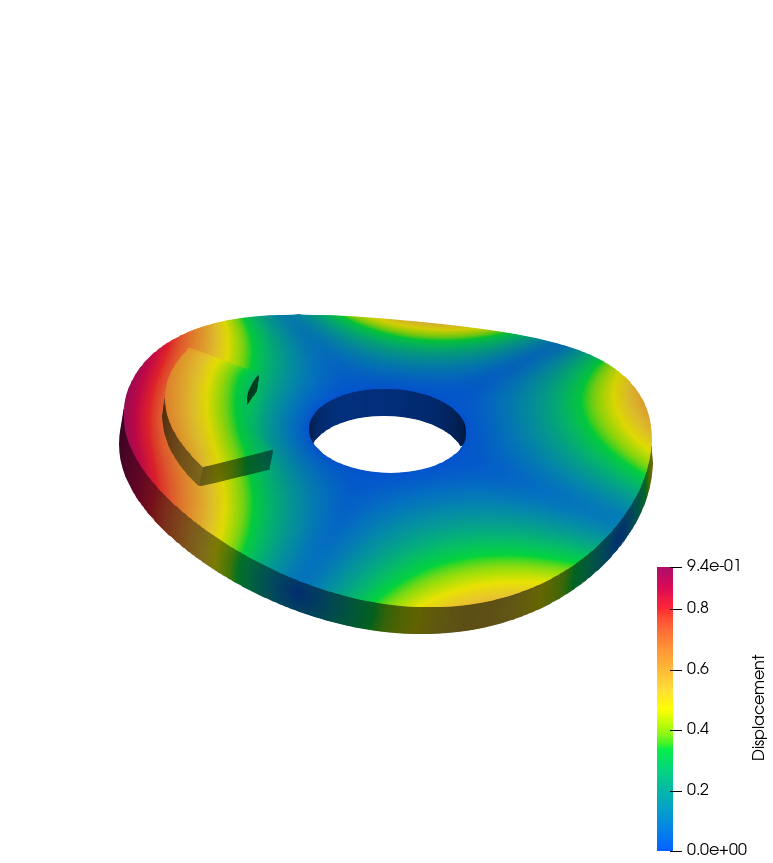
\includegraphics[scale=0.27]{Chapter1/Pictures/Shape_5.png}}
    \subfloat[Mode no. 26, Frequency:9245 Hz]{
    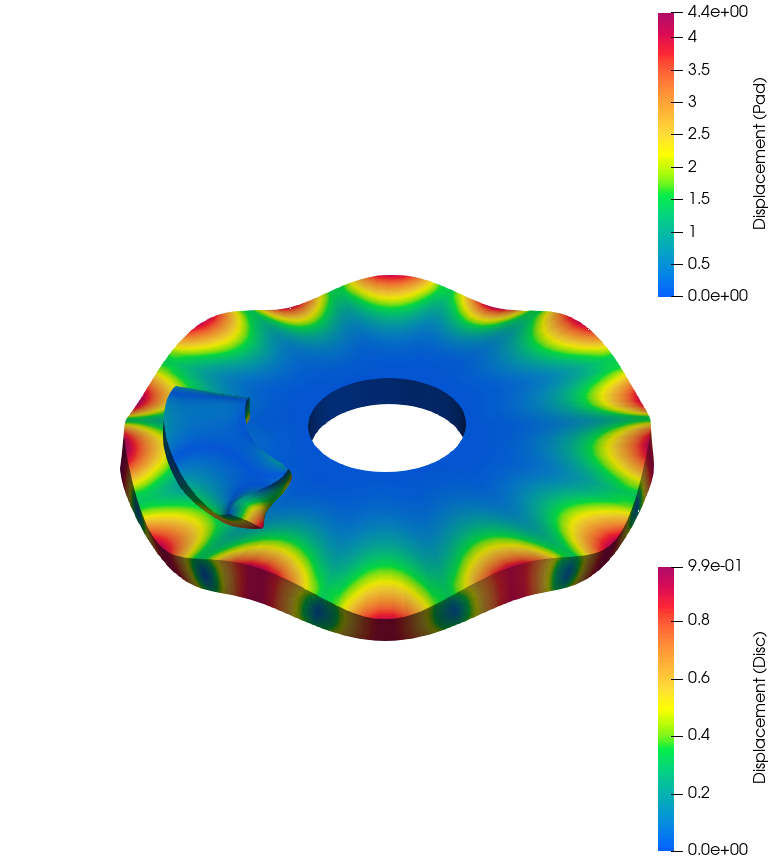
\includegraphics[scale=0.27]{Chapter1/Pictures/Shape_26.png}}
    \caption{Example of disc-pad stable modes}
    \label{fig:stable_modes}
\end{figure}

 \begin{figure}[h!]
    \centering
    \subfloat[Mode no. 45, Frequency:12236 Hz]{
    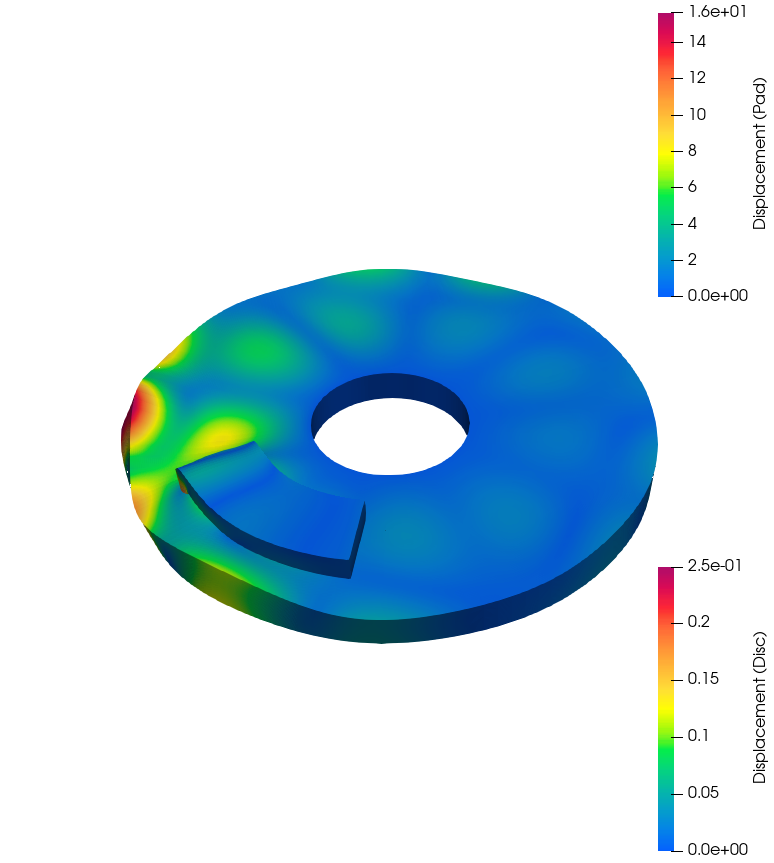
\includegraphics[scale=0.27]{Chapter1/Pictures/Shape_45.png}}
    \subfloat[Mode no. 82, Frequency:17259 Hz]{
    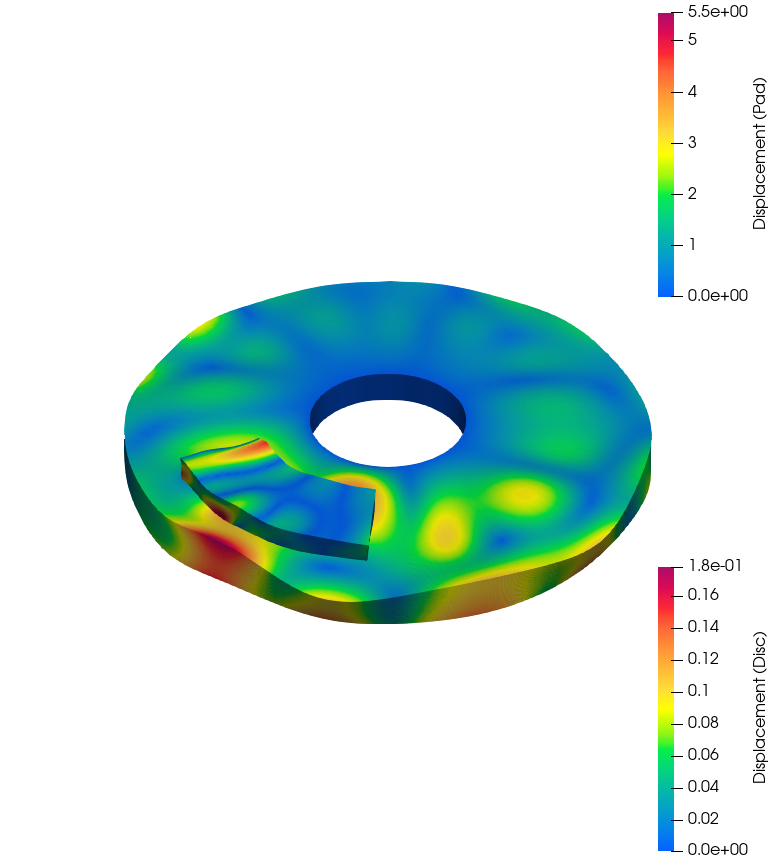
\includegraphics[scale=0.27]{Chapter1/Pictures/Shape_82.png}}
    \caption{Example of disc-pad unstable modes, where the displacement field is considered only for real-part of the eigenvector}
    \label{fig:unstable_modes}
\end{figure}

We discuss the empirical observations from the post-processing of mode shapes, even though the results are highly subjective and depend on the value of $p$ which is typically determined from experiments in the light of normal compliance.
Typically at low frequencies, the mode shape of the pad follows the shape of the disc with correspondence in displacement field at the contact interface. While at higher frequencies, the behaviour is complicated to understand, but relatively large difference in magnitude of displacement field between the disc and the pad was observed. 
Further, the unstable modes lead to definition of eigenvectors in complex-plane for displacement field, which was not considered for representation in Figure \ref{fig:unstable_modes}. 
For intuition, a complex eigenvalue with non-zero real and imaginary parts, defines the phase-lag in the displacement field for an eigenvector and hence, the stable equilibrium position of the displacement field for an eigenvector is never achieved simultaneously.\\

\subsubsection{Optimization criterion definition}

In the context of shape optimization, the idea is to define a criterion for optimization independent of the coefficient of friction ${\mu}$, such as to reduce the influence of ${\mu}$ in determining the shape. This is because the parameter $\mu$ is mostly uncertain in real world and also instabilities could be easily averted at lower values of ${\mu}$. Hence, to define a criterion which characterizes instability for a geometric shape $\bm X$ independent of ${\mu}$, we define the criterion as follows
 
 \begin{equation}
C_{\mathsf s}(\bm X)=\int_{{\mu}} max\{\Re(\bm \Lambda(\bm X,{\mu}))\}\,d{\mu}
    \label{eq:firststabcrit}
\end{equation}
 
where $\bm \Lambda=\{\lambda_1\cdots\lambda_{(.)}\}$ is a set of eigenvalues of the system. 
The criterion is essentially a black-box function defined by the maximum of the real part in $\bm \Lambda(\bm X)$ at a given value of ${\mu}$, integrated over ${\mu}$.
Typically, it can be too unrealistic or optimistic to minimise the criterion over the whole range of squeal frequency ($1$ to $16$ $KHz$) and hence, the set $\bm \Lambda$ can be chosen for a specific range of frequency.
This can also be a better strategy in defining meta-model for $C_{\mathsf s}$, since the meta-model can be more accurate in characterising the behaviour of modes over a specific range of frequency than the whole range.
Even though, no correlation can be implied between $\max\{\Re(\bm \Lambda(\bm X,{\mu}))\}$ and noise level, choosing $\max\{\Re(\bm \Lambda(\bm X,{\mu}))\}$ is essential to define some smoothness for $C_{\mathsf s}$ in optimisation. 
Hence the choice of $\max\{\Re(\bm \Lambda(\bm X,{\mu}))\}$ does not necessarily characterise noise level but the presence of instability which can be accounted for squeal noise. 
Nevertheless, the Utopian goal of $C_{\mathsf s}=0$ defines lack of instabilities and hence characterising noise level may not be a concern if such a goal could be reached in optimisation.\\

Evaluation of $C_{\mathsf s}$ can be computationally expensive, but with the aid of model reduction and parallel computing, it can be made to be efficient. In the following, we give the general frame-work for evaluating $C_{\mathsf s}$.

The reduced stiffness matrices of the multi-patch disc can be defined with C\&B method as

  \begin{equation}
 \mathbf{\hat{K}}^{\mathrm{(d)}}=\left[
\begin{array}{cccc}
  \mathcal{\hat I}^{(\mathrm d)} &0\\
  0&\mathbf{\hat{K}}_{\mathrm{vv}}^{(\mathrm d)} \\
\end{array}
\right] 
 \end{equation}

where the matrix is defined by the coordinates 
$\bm Z^{(\mathrm d)}= \left[\begin{array}{cc}
  \mathscr{M}^{(\mathrm d)} \\
  \bm U_{\mathrm{v}}^{(\mathrm d)} \end{array}\right]$
  , with $\bm U_{\mathrm{v}}^{(\mathrm d)}$ defining the degrees of freedom on $\Gamma_{C}^{(\mathrm d)}$ \footnote{It should be noted that in the context of multi-patch parameterisation, detailed in \S ,$\Gamma_{C}^{(\mathrm d)}$ corresponds to $\Gamma_{C}^{(\mathrm d_1)}$, where the contact interface is defined to be on $\Omega^{(\mathrm d_1)}$.}.
 The matrix is essentially the same in optimisation, when the optimisation is defined only for $\Omega^{\mathrm{p}}$. Hence, for a given definition of shape, the following matrix is computed
 
   \begin{equation}
 \mathbf{\hat{K}}^{\mathrm{(p)}}=\left[
\begin{array}{cccc}
  \mathcal{\hat I}^{(\mathrm p)} &0\\
  0&\mathbf{\hat{K}}_{\mathrm{vv}}^{(\mathrm p)} \\
\end{array}
\right] 
 \end{equation}
 
 The evaluation of $C_{\mathsf s}$ demands the definition of  $\mathbf{\hat{K}}^{\mathrm{(d-p)}}$ for several values of $\mu$. Since $\mu$ is the property of interface, the characteristics at the interface can be decoupled as interface degrees of freedom $\bm U_{\mathrm{v}}$ in C\&B reduced coordinates. For the definition of $\mathbf{\hat K}_F^{\mathrm{(a-b)}}$, $\mu$ can be factored out as  $\mu \mathbf{\hat K}_F^{\mathrm{(a-b)}}|_{\mu=1}$, where in this case with $\mu$ factored out,  $\mathbf{\hat K}_F^{\mathrm{(a-b)}}|_{\mu=1}$ can be interpreted as $\mathbf{\hat K}_F^{\mathrm{(a-b)}}$ computed with $\mu=1$. The idea is that for the evaluation of $C_{\mathsf s}$, with numerical integration defined over $\mu$, the matrix $\mathbf{\hat K}_F^{\mathrm{(a-b)}}$ does not need to be evaluated for discrete values of $\mu$, but instead $\mu$ can be defined as factor of $\mathbf{\hat K}_F^{\mathrm{(a-b)}}|_{\mu=1}$, where $\mathbf{\hat K}_F^{\mathrm{(a-b)}}$ in this case is computed only once with $\mu=1$.\\ 
 
 
The computational cost of evaluating $C_{\mathsf s}$ with numerical integration for discrete values of ${\mu}$ can be reduced through 
 parallel computation. The only varying parameter for parallelisation is $\mu$ for the definition of $\mathbf{\hat K}_F^{\mathrm{(a-b)}}$, hence the computation of the matrices  $\mathbf{\hat{M}}^{\mathrm{(p)}}$, $\mathbf{\hat{K}}^{\mathrm{(p)}}$, $\mathbf{\hat{K}}^{\mathrm{(d-p)}}_C$ and $\mathbf{\hat{K}}^{\mathrm{(d-p)}}_F|_{\mu=1}$ are achieved on single core. Further with $\mathbf{\hat{M}}^{\mathrm{(d)}}$ and $\mathbf{\hat{K}}^{\mathrm{(d)}}$ already computed, the reduced matrices of $\mathbf{\hat{M}}^\mathrm{(d-p)}$ and $\mathbf{\hat{K}}^\mathrm{(d-p)}$ can also be defined on single core as
 
  \begin{equation}
 \mathbf{\hat{M}}^{(d-p)}=\left[
\begin{array}{cc}
  {{\mathbf{\hat M}}}^{(d)} &0\\
  0&{\mathbf{\hat M}}^{(p)} \\
\end{array}
\right] 
 \end{equation}
 

 \begin{equation}
 \mathbf{\hat{K}}^{\mathrm{(d-p)}}_{\uplus C}=\left[
\begin{array}{cccc}
  \mathcal{\hat I}^{(\mathrm a)} &0&0&0\\
  0&\mathbf{\hat{K}}_{\mathrm{vv}}^{(\mathrm a)}+ {{\mathbf{\hat K}}}^{\mathrm{(\mathrm d)}}_C&0&{{\mathbf{\hat K}}}^{\mathrm{(d,p)}}_C \\
  0&0& \mathcal{\hat I}^{(\mathrm p)} &0 \\
  0& {{\mathbf{\hat K}}}^{\mathrm{(p,d)}}_C+{{\mathbf{\hat K}}}^{\mathrm{(p,d)}}_F&0&\mathbf{\hat{K}}_{\mathrm{vv}}^{(p)}+ {{\mathbf{\hat K}}}^{\mathrm{(p)}}_C\\
\end{array}
\right] 
 \end{equation}
 
 
 where the matrices are expressed in coordinates $\mathbf{Z}^{(d-p)}$. Similarly, the matrix $\mathbf{\hat{K}}^{\mathrm{(d-p)}}_F|_{\mu=1}$ can be expressed in  $\mathbf{Z}^{(d-p)}$ coordinates as
 
  \begin{equation}
 \mathbf{\hat{K}}^{\mathrm{(d-p)}}_{\cup F}|_{\mu=1}=\left[
\begin{array}{cccc}
0&0&0&0\\
0& {{\mathbf{\hat K}}}^{\mathrm{(d)}}_F|_{\mu=1}&0& {{\mathbf{\hat K}}}^{\mathrm{(d,p)}}_F|_{\mu=1}\\
0&0&0&0\\
0& {{\mathbf{\hat K}}}^{\mathrm{(p,d)}}_F|_{\mu=1}&0& {{\mathbf{\hat K}}}^{\mathrm{(p)}}_F|_{\mu=1}\\
\end{array}
\right] 
 \end{equation}

The evaluation of $C_{\mathsf s}$ with numerical integration can be expressed as

\begin{equation}
\int_{{\mu}}max\{\Re(\bm \Lambda(\bm X,{\mu}))\}\,d{\mu} \approx \sum_{{\mu}_{\mathsf i}\in [0,1]}max\{\Re(\bm \Lambda(\bm X,{\mu}_{\mathsf i}))\}\,w_{{\mathsf i}}
\end{equation}

where ${\mu}_{\mathsf i}$ can be spaced evenly in the interval $[0,1]$. Hence, on each parallel core, the matrix $ \mathbf{\hat{K}}^{\mathrm{(d-p)}}_{\uplus CF}$ can be computed as

\begin{equation}
\mathbf{\hat{K}}^{\mathrm{(d-p)}}_{\uplus CF} =  \mathbf{\hat{K}}^{\mathrm{(d-p)}}_{\uplus C}+\mu_{\mathsf i} \,\mathbf{\hat{K}}^{\mathrm{(d-p)}}_{\cup F}|_{\mu=1}
\end{equation}

Along with the definition of $\mathbf{\hat{K}}^{\mathrm{(d-p)}}_{\uplus CF}$, the computation in parallel cores is defined for Eq. \eqref{eq:char_eqn} in reduced coordinates, where in each core, the computation of the characteristics eigenvalue problem in reduced coordinates can be expressed as

\begin{equation}
 (\lambda^{2} \mathbf{\hat M}^{\mathrm{(d-p)}}+\mathbf{\hat{K}}^{\mathrm{(d-p)}}_{\uplus C}+\mu_{\mathsf i}\, \mathbf{\hat{K}}^{\mathrm{(d-p)}}_{\cup F}|_{\mu=1}) \Theta =0
\end{equation} 

This eventually leads to the evaluation of $max\{\Re(\bm \Lambda(\bm X,{\mu}_{\mathsf i}))\}$ in each parallel core and hence with the evaluation of  $max\{\Re(\bm \Lambda(\bm X,{\mu}_{\mathsf i}))\}$ on all parallel cores, $C_{\mathsf s}$ can be computed from $\sum_{{\mu}_{\mathsf i}\in [0,1]}max\{\Re(\bm \Lambda(\bm X,{\mu}_{\mathsf i}))\}\,w_{{\mathsf i}}$.


\iffalse
When defined through numerical integration, the criterion demands evaluation at several values of ${\mu}$ and hence is computationally expensive. But this can be evaded through taking advantage of parallel computation with reduced dynamical models using Craig-Bampton reduction, where the computation of the matrices in physical coordinates followed by dynamic model reduction are achieved on the main core. 


The only varying parameter in the parallel cores is $\boldsymbol{\mu}$ and hence, the calculation of the reduced friction matrix $\mathbf{\hat{K}}^f_{d-p}$ matrix --i.e., the reduced matrix  represented in the Craig-Bampton coordinates-- is defined with $\bm{\mu} = 1$ on the main core and the parallelization is defined for distinct values of $\bm{\mu}$ for $\bm{\mu} \mathbf{\hat{K}}^f_{d-p}$. This means that in addition to the definition of $\bm{\mu} \mathbf{\hat{K}}^f_{d-p}$, the computation on the parallel cores is limited to solving the eigenvalue problem \eqref{eq:char_eqn} with the reduced dynamical model for evaluation of the criterion \eqref{eq:firststabcrit}, which makes it computationally efficient.
\fi

